%% abtex2-modelo-trabalho-academico.tex, v-1.9.7 laurocesar
%% Copyright 2012-2018 by abnTeX2 group at http://www.abntex.net.br/ 
%%
%% This work may be distributed and/or modified under the
%% conditions of the LaTeX Project Public License, either version 1.3
%% of this license or (at your option) any later version.
%% The latest version of this license is in
%%   http://www.latex-project.org/lppl.txt
%% and version 1.3 or later is part of all distributions of LaTeX
%% version 2005/12/01 or later.
%%
%% This work has the LPPL maintenance status `maintained'.
%% 
%% The Current Maintainer of this work is the abnTeX2 team, led
%% by Lauro César Araujo. Further information are available on 
%% http://www.abntex.net.br/
%%
%% This work consists of the files abntex2-modelo-trabalho-academico.tex,
%% abntex2-modelo-include-comandos and abntex2-modelo-references.bib
%%

% ------------------------------------------------------------------------
% ------------------------------------------------------------------------
% abnTeX2: Modelo de Trabalho Academico (tese de doutorado, dissertacao de
% mestrado e trabalhos monograficos em geral) em conformidade com 
% ABNT NBR 14724:2011: Informacao e documentacao - Trabalhos academicos -
% Apresentacao
% ------------------------------------------------------------------------
% ------------------------------------------------------------------------

\documentclass[
	hyphens,
	% -- opções da classe memoir --
	12pt,				% tamanho da fonte
	openright,			% capítulos começam em pág ímpar (insere página vazia caso preciso)
	twoside,			% para impressão em recto e verso. Oposto a oneside
	a4paper,			% tamanho do papel. 
	% -- opções da classe abntex2 --
	%chapter=TITLE,		% títulos de capítulos convertidos em letras maiúsculas
	%section=TITLE,		% títulos de seções convertidos em letras maiúsculas
	%subsection=TITLE,	% títulos de subseções convertidos em letras maiúsculas
	%subsubsection=TITLE,% títulos de subsubseções convertidos em letras maiúsculas
	% -- opções do pacote babel --
	english,			% idioma adicional para hifenização
	brazil				% o último idioma é o principal do documento
	]{abntex2}

% ---
% Pacotes básicos 
% ---
\usepackage{lmodern}			% Usa a fonte Latin Modern			
\usepackage[T1]{fontenc}		% Selecao de codigos de fonte.
\usepackage[utf8]{inputenc}		% Codificacao do documento (conversão automática dos acentos)
\usepackage{indentfirst}		% Indenta o primeiro parágrafo de cada seção.
\usepackage{color}				% Controle das cores
\usepackage{graphicx}			% Inclusão de gráficos
\usepackage{microtype} 			% para melhorias de justificação
\usepackage{longtable}
\usepackage{graphicx}
\usepackage{subfig}
\captionsetup[subfigure]{position=b}
\usepackage[locale=FR]{siunitx}
\sisetup{detect-all, math-rm = \ensuremath, math-micro = \symup{μ}}
\usepackage{tabularx}
\newcolumntype{Y}{>{\centering\arraybackslash}X}
\usepackage{float}
\usepackage{amstext}
\usepackage[space]{grffile}
% ---
		
% ---
% Pacotes adicionais, usados apenas no âmbito do Modelo Canônico do abnteX2
% ---
\usepackage{lipsum}				% para geração de dummy text
% ---

% ---
% Pacotes de citações
% ---
\usepackage[brazilian,hyperpageref]{backref}	 % Paginas com as citações na bibl
\usepackage[alf]{abntex2cite}	% Citações padrão ABNT
%\usepackage[style=abnt, backref=true]{biblatex}
%\addbibresource{library.bib}        
% --- 
% CONFIGURAÇÕES DE PACOTES
% --- 

% ---
% Configurações do pacote backref
% Usado sem a opção hyperpageref de backref
\renewcommand{\backrefpagesname}{Citado na(s) página(s):~}
% Texto padrão antes do número das páginas
\renewcommand{\backref}{}
% Define os textos da citação
\renewcommand*{\backrefalt}[4]{
	\ifcase #1 %
		Nenhuma citação no texto.%
	\or
		Citado na página #2.%
	\else
		Citado #1 vezes nas páginas #2.%
	\fi}%
% ---

\newcommand{\refanexo}[1]{\hyperref[#1]{Anexo~\ref{#1}}}

% ---
% Mudando a capa
\renewcommand{\imprimircapa}{
	\begin{capa}
		\center
		Universidade de São Paulo
		\par
		Instituto de Astronomia, Geofísica e Ciências Atmosféricas
		\par
		Departamento de Ciências Atmosféricas
		
		\vspace*{3cm}
		
		{\ABNTEXchapterfont\large\imprimirautor}
		
		\vspace*{4cm}
		\begin{center}
			\ABNTEXchapterfont\bfseries\LARGE\imprimirtitulo
		\end{center}
		\vfill
		
		\large\imprimirlocal
		
		\large\imprimirdata
		
		\vspace*{1cm}
	\end{capa}
}

\addto\captionsbrazil{%
	\renewcommand{\listfigurename}%
	{Lista de figuras}%
}

% ---
% Informações de dados para CAPA e FOLHA DE ROSTO
% ---
\titulo{Microfísica, Cinemática e Eletrificação em Tempestades Tropicais que geram Granizo durante o Projeto SOS-CHUVA}
\autor{Camila da Cunha Lopes}
\local{São Paulo}
\data{2019}
%\orientador{Prof\textordfeminine\:Dr\textordfeminine\:Rachel Ifanger Albrecht}
%\instituicao{%
%  Universidade de São Paulo
%  \par
%  Instituto de Astronomia, Geofísica e Ciências Atmosféricas
%  \par
%  Departamento de Ciências Atmosféricas}
\tipotrabalho{Dissertação (Mestrado)}
% O preambulo deve conter o tipo do trabalho, o objetivo, 
% o nome da instituição e a área de concentração 
\preambulo{%
	Dissertação apresentada ao Departamento de Ciências Atmosféricas do Instituto de Astronomia, Geofísica e Ciências Atmosféricas da Universidade de São Paulo como requisito parcial para a obtenção do título de Mestre em Ciências.
	\par \vspace{1cm}
	Área de Concentração: Meteorologia
	\par
	\mbox{Orientadora: Prof\textordfeminine\:Dr\textordfeminine\:Rachel Ifanger Albrecht}
}
% ---


% ---
% Configurações de aparência do PDF final

% alterando o aspecto da cor azul
\definecolor{blue}{RGB}{41,5,195}

% informações do PDF
\makeatletter
\hypersetup{
     	%pagebackref=true,
		pdftitle={\@title}, 
		pdfauthor={\@author},
%    	pdfsubject={\imprimirpreambulo},
	    pdfcreator={LaTeX with abnTeX2},
		pdfkeywords={abnt}{latex}{abntex}{abntex2}{trabalho acadêmico}, 
		colorlinks=true,       		% false: boxed links; true: colored links
    	linkcolor=blue,          	% color of internal links
    	citecolor=blue,        		% color of links to bibliography
    	filecolor=magenta,      		% color of file links
		urlcolor=blue,
		bookmarksdepth=4
}
\makeatother
% --- 

% ---
% Posiciona figuras e tabelas no topo da página quando adicionadas sozinhas
% em um página em branco. Ver https://github.com/abntex/abntex2/issues/170
\makeatletter
\setlength{\@fptop}{5pt} % Set distance from top of page to first float
\makeatother
% ---

% ---
% Possibilita criação de Quadros e Lista de quadros.
% Ver https://github.com/abntex/abntex2/issues/176
%
%\newcommand{\quadroname}{Quadro}
%\newcommand{\listofquadrosname}{Lista de quadros}
%
%\newfloat[chapter]{quadro}{loq}{\quadroname}
%\newlistof{listofquadros}{loq}{\listofquadrosname}
%\newlistentry{quadro}{loq}{0}
%
%% configurações para atender às regras da ABNT
%\setfloatadjustment{quadro}{\centering}
%\counterwithout{quadro}{chapter}
%\renewcommand{\cftquadroname}{\quadroname\space} 
%\renewcommand*{\cftquadroaftersnum}{\hfill--\hfill}
%
%\setfloatlocations{quadro}{hbtp} % Ver https://github.com/abntex/abntex2/issues/176
% ---

% --- 
% Espaçamentos entre linhas e parágrafos 
% --- 

% O tamanho do parágrafo é dado por:
\setlength{\parindent}{1.3cm}

% Controle do espaçamento entre um parágrafo e outro:
\setlength{\parskip}{0.2cm}  % tente também \onelineskip

% ---
% compila o indice
% ---
\makeindex
% ---

% ----
% Início do documento
% ----
\begin{document}

% Seleciona o idioma do documento (conforme pacotes do babel)
%\selectlanguage{english}
\selectlanguage{brazil}

% Retira espaço extra obsoleto entre as frases.
\frenchspacing 

% ----------------------------------------------------------
% ELEMENTOS PRÉ-TEXTUAIS
% ----------------------------------------------------------
% \pretextual

% ---
% Capa
% ---
\imprimircapa

% ---

% ---
% Folha de rosto
% (o * indica que haverá a ficha bibliográfica)
% ---
\imprimirfolhaderosto
% ---

% ---
% Inserir a ficha bibliografica
% ---

% Isto é um exemplo de Ficha Catalográfica, ou ``Dados internacionais de
% catalogação-na-publicação''. Você pode utilizar este modelo como referência. 
% Porém, provavelmente a biblioteca da sua universidade lhe fornecerá um PDF
% com a ficha catalográfica definitiva após a defesa do trabalho. Quando estiver
% com o documento, salve-o como PDF no diretório do seu projeto e substitua todo
% o conteúdo de implementação deste arquivo pelo comando abaixo:
%
% \begin{fichacatalografica}
%     \includepdf{fig_ficha_catalografica.pdf}
% \end{fichacatalografica}

%\begin{fichacatalografica}
%	\sffamily
%	\vspace*{\fill}					% Posição vertical
%	\begin{center}					% Minipage Centralizado
%	\fbox{\begin{minipage}[c][8cm]{13.5cm}		% Largura
%	\small
%	\imprimirautor
%	%Sobrenome, Nome do autor
%	
%	\hspace{0.5cm} \imprimirtitulo  / \imprimirautor. --
%	\imprimirlocal, \imprimirdata-
%	
%	\hspace{0.5cm} \thelastpage p. : il. (...) ; 30 cm.\\
%	
%	\hspace{0.5cm} \imprimirorientadorRotulo~\imprimirorientador\\
%	
%	\hspace{0.5cm}
%	\parbox[t]{\textwidth}{\imprimirtipotrabalho~--~\imprimirinstituicao,
%	\imprimirdata.}\\
%	
%	\hspace{0.5cm}
%		1. Palavra-chave1.
%		2. Palavra-chave2.
%		2. Palavra-chave3.
%		I. Orientador.
%		II. Universidade xxx.
%		III. Faculdade de xxx.
%		IV. Título 			
%	\end{minipage}}
%	\end{center}
%\end{fichacatalografica}
% ---

% ---
% Inserir errata, folha de aprovação, dedicatória, agradecimentos, epígrafe
% ---

% ---
% Inserir errata
% ---
%\begin{errata}
%Elemento opcional da \citeonline[4.2.1.2]{NBR14724:2011}. Exemplo:
%
%\vspace{\onelineskip}
%
%FERRIGNO, C. R. A. \textbf{Tratamento de neoplasias ósseas apendiculares com
%reimplantação de enxerto ósseo autólogo autoclavado associado ao plasma
%rico em plaquetas}: estudo crítico na cirurgia de preservação de membro em
%cães. 2011. 128 f. Tese (Livre-Docência) - Faculdade de Medicina Veterinária e
%Zootecnia, Universidade de São Paulo, São Paulo, 2011.
%
%\begin{table}[htb]
%\center
%\footnotesize
%\begin{tabular}{|p{1.4cm}|p{1cm}|p{3cm}|p{3cm}|}
%  \hline
%   \textbf{Folha} & \textbf{Linha}  & \textbf{Onde se lê}  & \textbf{Leia-se}  \\
%    \hline
%    1 & 10 & auto-conclavo & autoconclavo\\
%   \hline
%\end{tabular}
%\end{table}
%
%\end{errata}
% ---

% ---
% Inserir folha de aprovação
% ---

% Isto é um exemplo de Folha de aprovação, elemento obrigatório da NBR
% 14724/2011 (seção 4.2.1.3). Você pode utilizar este modelo até a aprovação
% do trabalho. Após isso, substitua todo o conteúdo deste arquivo por uma
% imagem da página assinada pela banca com o comando abaixo:
%
% \begin{folhadeaprovacao}
% \includepdf{folhadeaprovacao_final.pdf}
% \end{folhadeaprovacao}
%
%\begin{folhadeaprovacao}
%
%  \begin{center}
%    {\ABNTEXchapterfont\large\imprimirautor}
%
%    \vspace*{\fill}\vspace*{\fill}
%    \begin{center}
%      \ABNTEXchapterfont\bfseries\Large\imprimirtitulo
%    \end{center}
%    \vspace*{\fill}
%    
%    \hspace{.45\textwidth}
%    \begin{minipage}{.5\textwidth}
%        \imprimirpreambulo
%    \end{minipage}%
%    \vspace*{\fill}
%   \end{center}
%        
%   Trabalho aprovado. \imprimirlocal, 24 de novembro de 2012:
%
%   \assinatura{\textbf{\imprimirorientador} \\ Orientador} 
%   \assinatura{\textbf{Professor} \\ Convidado 1}
%   \assinatura{\textbf{Professor} \\ Convidado 2}
%   %\assinatura{\textbf{Professor} \\ Convidado 3}
%   %\assinatura{\textbf{Professor} \\ Convidado 4}
%      
%   \begin{center}
%    \vspace*{0.5cm}
%    {\large\imprimirlocal}
%    \par
%    {\large\imprimirdata}
%    \vspace*{1cm}
%  \end{center}
%  
%\end{folhadeaprovacao}
% ---

% ---
% Dedicatória
% ---
%\begin{dedicatoria}
%	\vspace*{\fill}
%	\centering
%	\noindent
%	\textit{ Este trabalho é dedicado às crianças adultas que,\\
%		quando pequenas, sonharam em se tornar cientistas.} \vspace*{\fill}
%\end{dedicatoria}
% ---

% ---
% Agradecimentos
% ---
\begin{agradecimentos}
   À minha orientadora, Prof\textordfeminine\:Dr\textordfeminine\:Rachel Ifanger Albrecht, por todas as oportunidades dentro e fora da pesquisa, contribuindo imensamente para o meu crescimento pessoal e profissional.
   À Fundação de Amparo à Pesquisa do Estado de São Paulo (FAPESP), sob o processo n\textordmasculine\:2017/06075-3 (vinculado ao processo n\textordmasculine\:2015/14497-0) pelo apoio financeiro para a realização da pesquisa e apresentação em congresso internacional.
   À Secretaria e Seção de Informática do Departamento de Ciências Atmosféricas (DCA-IAG) pela ajuda técnica e burocrática.
   À toda equipe do Projeto SOS-CHUVA pela dedicação na instalação, manutenção, desenvolvimento e divulgação que permitiram que esse trabalho pudesse ser feito.
   Ao Prof\textordmasculine\:Dr. Lawrence D. Carey, Msc. Sarah Stough e demais colegas do grupo de trabalho do Departamento de Ciências Atmosféricas da Universidade do Alabama em Huntsville (UAH) que me auxiliaram no processamento da recuperação de vento por Multi-Doppler durante a visita à universidade.
   Aos amigos e colegas de departamento, especialmente Isabela Siqueira, Victória Peli e Alan Rosales, pela companhia e apoio, principalmente nas (muitas) horas difíceis.
   E, acima de tudo, à minha família, Janice, Fernando e Yukio, por serem meu grande alicerce durante esses dois anos.
\end{agradecimentos}
% ---

% ---
% Epígrafe
% ---
\begin{epigrafe}
	\vspace*{\fill}
	\begin{flushright}
		\begin{figure}[hb]
			\includegraphics[width=0.5\columnwidth,right]{figs/cat_meme.jpg}
		\end{figure}
		\textit{Fonte: \citeonline{Vernessa2017}.}
%		\textit{``Não vos amoldeis às estruturas deste mundo, \\
%			mas transformai-vos pela renovação da mente, \\
%			a fim de distinguir qual é a vontade de Deus: \\
%			o que é bom, o que Lhe é agradável, o que é perfeito.\\
%			(Bíblia Sagrada, Romanos 12, 2)}
	\end{flushright}
\end{epigrafe}
% ---

% ---
% RESUMOS
% ---

% ---
% RESUMOS
% ---

% resumo em português
\setlength{\absparsep}{18pt} % ajusta o espaçamento dos parágrafos do resumo
\begin{resumo}
 Esta dissertação analisou tempestades que produziram granizo na Região Metropolitana de Campinas com o objetivo de identificar fatores determinantes para a produção e precipitação de granizo. De forma inédita, uma rede de detecção de granizo instalada na região permitiu a identificação e determinação das intensidades das tempestades entre 2016 e 2017. O ciclo de vida, estrutura microfísica e cinemática de casos específicos foram estudados usando três radares meteorológicos instalados no estado de São Paulo e uma rede de detecção de raios, com ferramentas como rastreamento de sistemas convectivos, identificação de hidrometeoros e recuperação de vento tridimensional por Multi-Doppler. Comparando com escalas de intensidade de granizo aplicadas ao continente europeu, os casos analisados apresentaram intensidade baixa, com granizo de no máximo $22,4\:mm$ de diâmetro. O caso de 2017-03-14 apresentou o tempo de vida mais longo ($6,2\:h$), queda de granizo em duas localidades (com diâmetro máximo de $11,8\:mm$) e atividade elétrica mais intensa (taxa máxima de 107 (31) $flashes\:min^{-1}$ IC (CG)), enquanto que o caso de 2017-11-15, com tempo de vida mais curto ($2,2\:h$), apresentou baixa atividade elétrica (total de 46 (20) \textit{flashes} IC (CG)) porém com queda de granizo mais intensa. Todas as quedas de granizo dos casos específicos citados anteriormente estão associadas a uma extensa coluna de granizo identificada pelo radar polarimétrico e correntes ascendentes de até $30\:ms^{-1}$ antes do evento; o granizo maior no caso de 2017-11-15 possivelmente tem contribuição da precipitação na forma líquida (associada à correntes descendentes mais intensas) que previne a diminuição de tamanho do granizo ao mesmo tempo que contribui para o seu crescimento mesmo abaixo da base da nuvem.

 \textbf{Palavras-chave}: Granizo. Microfísica de Nuvens. Multi-Doppler. São Paulo.
\end{resumo}

% resumo em inglês
\begin{resumo}[Abstract]
 \begin{otherlanguage*}{english}
   This dissertation analyzed hail producing storms on the Metropolitan Region of Campinas to identify key factors for hailfall occurence. For the first time, a hail detection network installed in the region allowed the identification and determination of thunderstorm intensity in the 2016-2017 period. The life cycle, microphysical structure and kinematics of specific cases were studied  using three meteorological radars installed in São Paulo state and a lightning detection network, with tools such as tracking of convective systems, hydrometeor identification and Multi-Doppler 3D wind retrieval. The analyzed cases had low hailfall intensity when compared with scales applied in Europe, with $22.4\:mm$ maximum hail diameter. The 2017-03-14 case presented the longest lifetime ($6.2\:h$), hailfall in two locations ($11.8\:mm$ maximum hail diameter) and the most intense lightning activity (107 (31) $flashes\:min^{-1}$ IC (CG) maximum rate), while the 2017-11-15 case, with a shorter lifetime ($2.2\:h$), presented low electrical activity (46 (20) \textit{flashes} IC (CG) total) with the most intense hailfall. All hailfall cases of the specific cases mentioned earlier are associated with a extensive hail column identified by the polarimetric radar and up to $30\:ms^{-1}$ updrafts before the events; the bigger hail in the 2017-11-15 case posibly had the contribution of liquid precipitation (associated with larger downdrafts) which prevents hail size decrease as well as contributes to its growth below the cloud base.

   \textbf{Keywords}: Hail. Cloud Microphysics. Multi-Doppler. São Paulo.
 \end{otherlanguage*}
\end{resumo}

% ---
% inserir lista de ilustrações
% ---
\pdfbookmark[0]{\listfigurename}{lof}
\listoffigures*
\cleardoublepage
% ---

% ---
% inserir lista de quadros
% ---
%\pdfbookmark[0]{\listofquadrosname}{loq}
%\listofquadros*
%\cleardoublepage
% ---

% ---
% inserir lista de tabelas
% ---
\pdfbookmark[0]{\listtablename}{lot}
\listoftables*
\cleardoublepage
% ---

% ---
% inserir lista de abreviaturas e siglas
% ---
% ---
% inserir lista de abreviaturas e siglas
% ---
\begin{siglas}
  \item[RMC] Região Metropolitana de Campinas
  \item[SP] São Paulo
  \item[UNICAMP] Universidade Estadual de Campinas
  \item[LIM] Laboratório de Instrumentação Meteorológica
  \item[CPTEC] Centro de Previsão de Tempo e Estudos Climáticos
  \item[INPE] Instituto Nacional de Pesquisas Espaciais
  \item[DCA] Departamento de Ciências Atmosféricas
  \item[IAG] Instituto de Astronomia, Geofísica e Ciências Atmosféricas
  \item[USP] Universidade de São Paulo
  \item[ANELFA] \textit{Association Nationale d'Etude et de Lutte contre les Fléaux Atmosphériques}
  \item[TORRO] \textit{Tornado and Storm Research Organisation}
  \item[FCTH] Fundação Centro Tecnológico de Hidráulica
  \item[SR] São Roque (radar)
  \item[XPOL] Radar polarimétrico Banda-X
  \item[Py-ART] \textit{Python ARM Radar Toolkit}
  \item[DECEA] Departamento de Controle do Espaço Aéreo
  \item[CAPPI] Constant Altitude Plan Position Indicator
  \item[ForTraCC] \textit{Forecast and Tracking the Evolution of Cloud Clusters}
  \item[3DVAR] \textit{3D Variational Analysis}
  \item[4DD] \textit{Four-Dimensional Doppler Dealising Scheme}
  \item[BrasilDAT] Sistema Brasileiro de Detecção de Descargas Elétricas
  \item[LF] \textit{Low Frequency}
  \item[HF] \textit{High Frequency}
  \item[IC] \textit{Intra-Cloud}
  \item[CG] \textit{Cloud-to-Ground}
  \item[ELAT] Grupo de Eletricidade Atmosférica
  \item[CCST] Centro de Ciência do Sistema Terrestre
  \item[DBSCAN] \textit{Density-Based Spatial Clustering of Application with Noise}
  \item[ECMWF] \textit{European Centre for Medium-Range Weather Forecasts}
  \item[CDS] \textit{Climate Data Store}
  \item[CCCS] \textit{Copernicus Climate Change Service}
  \item[ABI] \textit{Advanced Baseline Imager}
  \item[GLM] \textit{Geoestationary Lightning Mapper}
  \item[NOAA] \textit{National Oceanic and Atmospheric Administration}
  \item[AWS] \textit{Amazon Web Services}
  \item[CAPE] \textit{Convective Available Potential Energy}
  \item[CIN] \textit{Convective Inibition}
  \item[ZCAS] Zona de Convergência do Atlântico Sul
\end{siglas}
% ---

% ---

% ---
% inserir lista de símbolos
% ---
%\begin{simbolos}
%  \item[$ \Gamma $] Letra grega Gama
%  \item[$ \Lambda $] Lambda
%  \item[$ \zeta $] Letra grega minúscula zeta
%  \item[$ \in $] Pertence
%\end{simbolos}
% ---

% ---
% inserir o sumario
% ---
\pdfbookmark[0]{\contentsname}{toc}
\tableofcontents*
\cleardoublepage
% ---


% ----------------------------------------------------------
% ELEMENTOS TEXTUAIS
% ----------------------------------------------------------
\textual
%\setcounter{page}{1}

% ----------------------------------------------------------
% Introdução 

% ----------------------------------------------------------
% Introdução (exemplo de capítulo sem numeração, mas presente no Sumário)
% ----------------------------------------------------------
\chapter{Introdução}
% ----------------------------------------------------------

[sobre granizo, severidade no sudeste - CHUVA, Nascimento, etc]

[sobre granizo em SP - Ceped]

[sobre o SOS-CHUVA]
"Como parte do Projeto SOS-CHUVA (FAPESP 2015/14497-0), pela primeira vez no
Brasil, temos medições in-situ da precipitação de granizo (dezembro de 2016 até o presente). Essas
medidas são compostas de distribuição de tamanho de granizo capturado por uma rede de detecçãp
de granizo (hailpad) instalada na Região Metropolitana de Campinas (RMC). Informações de
granizo combinadas com dados volumétricos de radar e descargas elétricas permitem um estudo
detalhado da microfísica, cinemática e eletrificação de granizo produzindo tempestades tropicais
durante o experimento de campo SOS-CHUVA"


\section{Objetivos}

O objetivo deste trabalho é explorar aspectos físicos de tempestades tropicais que geram granizo, de forma a caracterizar seus processos de formação e intensificação. A partir da cinemática convectiva e atividade elétrica, identificaremos fatores determinantes para que tempestades tropicais produzam granizo com tamanho suficiente para precipitar.

% Referencial teórico
\chapter{Referencial Teórico}\label{teoria}

\section{Processos de Formação do Granizo}

\section{Granizo e Eletrificação de Tempestades}\label{granizo_eletrificacao}

\section{Tempestades de Granizo na América do Sul}

\section{Usando Radares Meteorológicos para Estudar a Cinemática das Tempestades}



% Dados e Métodos
\chapter{Material e Métodos}\label{database}

A partir da base de dados do Projeto SOS-CHUVA, cinco casos foram selecionados, onde houve queda de granizo medida pela rede de hailpads (\autoref{hailpads}). A \autoref{tabela_casos} mostra uma breve descrição de cada caso.

\begin{table}[htb]
	\IBGEtab{%
		\caption{Descrição dos casos selecionados para análise}%
		\label{tabela_casos}
	}{%
		\begin{tabularx}{\textwidth}{cYYY}
			\toprule
			Caso & Descrição & Regiões Afetadas & Tipo de Severidade \\
			\midrule
			2016-12-25 & Condições instáveis na região levou à formação de diversos sistemas convectivos & Campinas, Vale do Paraíba, São Carlos & Rajadas de vento, granizo \\
			\midrule 
			2017-01-31 & Linha de Instabilidade formada a partir de condições de calor e umidade favoráveis & Sorocaba, Itu, Araraquara & Granizo \\
			\midrule 
			2017-03-14 & Aquecimento da superfície e convergência de umidade associada a uma frente fria no oceano favoreceu a formação de sistemas convectivos no centro do estado & Campinas, Indaiatuba, Jacareí & Granizo \\
			\midrule 
			2017-11-15 & Condições localmente favoráveis levaram à formação de sistemas convectivos isolados no centro do estado de SP & Indaiatuba, Bebedouro & Granizo \\
			\midrule 
			2017-11-16 & Escoamento do Jato de Baixos Níveis no centro-sul do país possibilitou condições de calor e umidade favoráveis para a formação de sistemas convectivos em todo o estado & Lorena, Ribeirão Preto, Campinas, São Paulo, Itapeva & Rajadas de vento, granizo \\
			\bottomrule
		\end{tabularx}%
	}{%
		\fonte{Adaptado de \url{https://topicssoschuva.blogspot.com.br/2017/03/summary-of-case-studies.html}.}%
	}
\end{table}


\section{Rede de Detecção de Granizo}\label{hailpads}

Dentro do Projeto SOS-CHUVA, uma rede de detecção de granizo foi instalada na Região Metropolitana de Campinas, dentro da cobertura do radar meteorológico Banda-X instalado na UNICAMP (XPOL). Como mostrado na Figura\autoref{rede_hailpads}, a rede foi composta por 24 localidades, com maior densidade de pontos nas cidades de Campinas e Indaiatuba. O instrumento, chamado de hailpad, é composto por uma placa de isopor usado para isolamento coberta por uma folha de alumínio e fixada em um suporte de ferro aproximadamente 1,5 m acima da superfície. Na Figura\autoref{hailpad_indaiatuba} é possível observar uma placa instalada em Indaiatuba.

\begin{figure}[htb]
	\begin{center}
		\caption{(a) Rede de hailpads instalada na Região Metropolitana de Campinas com a localização e cobertura de 80 km do radar XPOL. (b) Hailpad instalado na cidade de Indaiatuba, na localização indicada com a seta em (a).} 
		\label{overview_hailpads}
		\subfloat[]{\includegraphics[width=0.75\columnwidth]{figs/hailpad_network.jpg}
			\label{rede_hailpads}}
		\ \
		\subfloat[]{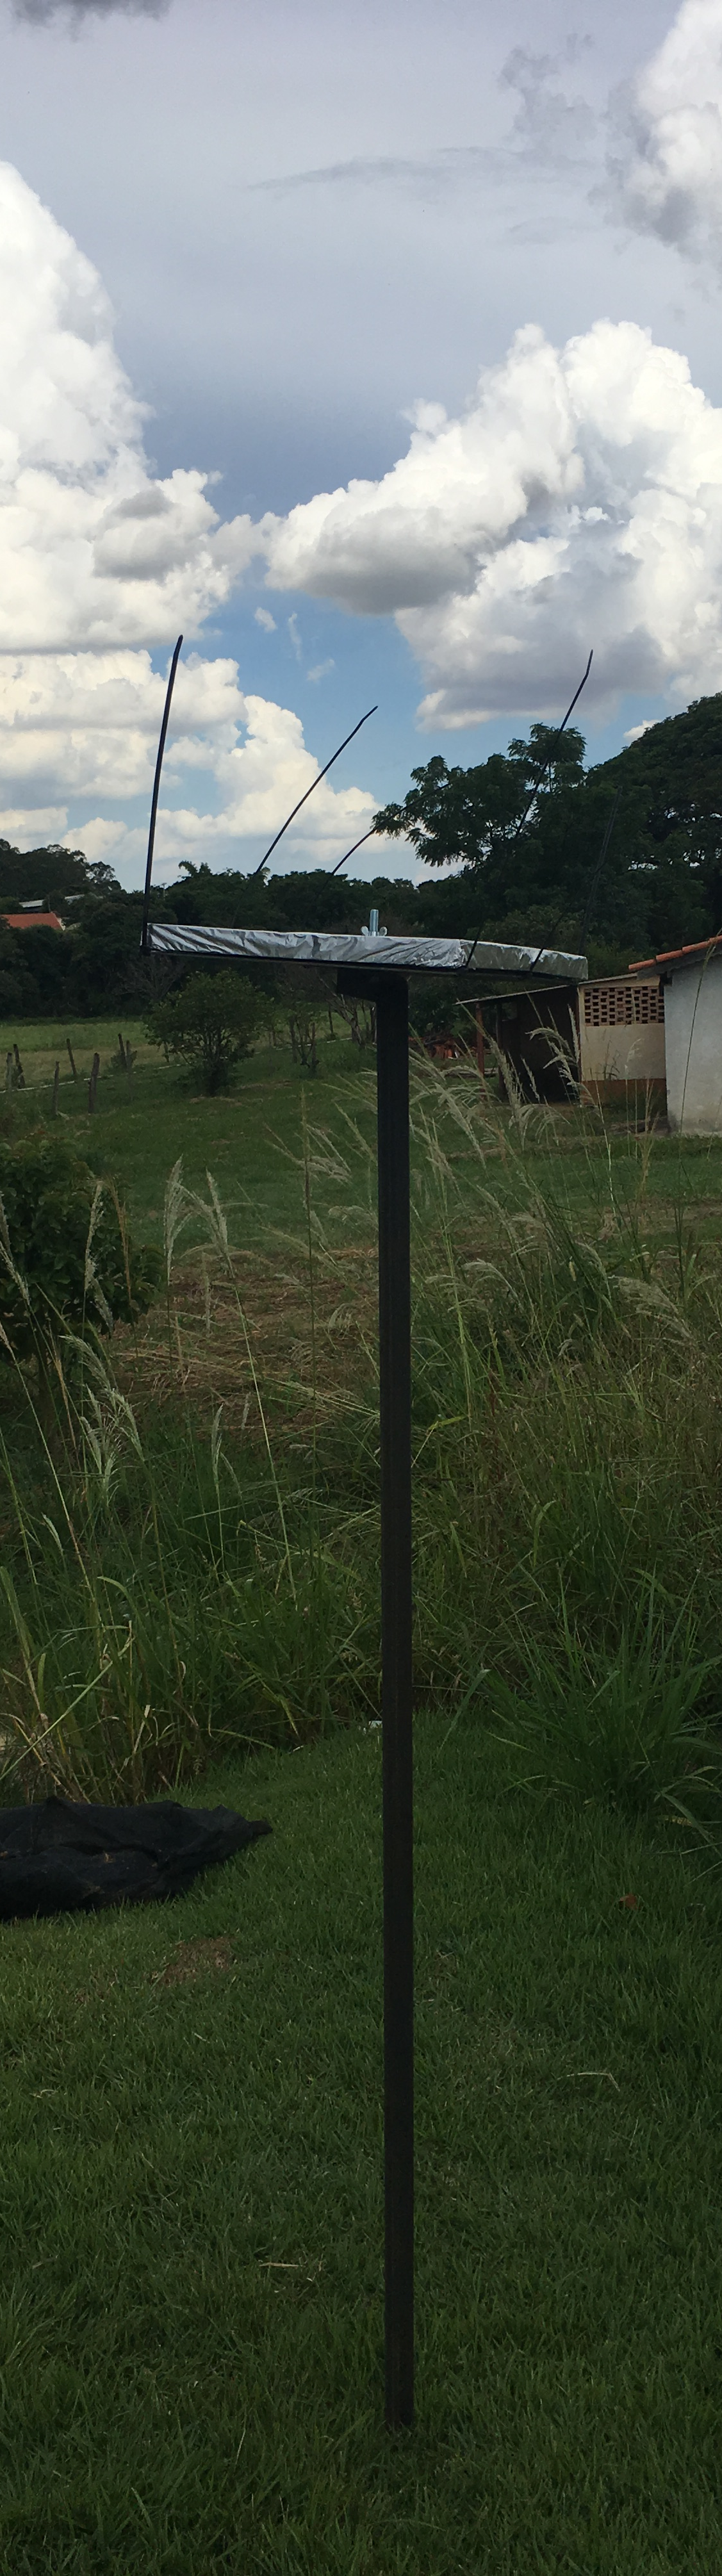
\includegraphics[width=0.158\columnwidth]{figs/hailpad.png}
			\label{hailpad_indaiatuba}}\\
		\legend{Fonte: Produzido pela autora.}
	\end{center}
\end{figure}

Os casos descritos na \autoref{tabela_casos} foram selecionados com base nos registros dos hailpads dentro da rede. A \autoref{tabela_hailpads} mostra a localização das placas e os grupos que mediram a distribuição de tamanho de granizo, sendo eles: Laboratório de Instrumentação Meteorológica (LIM/CPTEC-INPE) e Departamento de Ciências Atmosféricas (DCA/IAG-USP). Não houve registro da localização exata da placa C004. 

\begin{table}[htb]
	\IBGEtab{%
		\caption{Descrição dos hailpads coletados para cada caso.}%
		\label{tabela_hailpads}
	}{%
		\begin{tabularx}{\textwidth}{YYYY}
			\toprule
			Data do evento & Código do hailpad coletado & Localização & Medido por \\
			\midrule 
			2016-12-25 & C002 & Campinas & IAG, LIM \\
			\midrule 
			2017-01-31 & C003 & Campinas & IAG, LIM \\ 
			 & C004 & Arredores de Campinas & IAG, LIM \\
			\midrule 
			2017-03-14 & C001 & Cosmópolis & IAG \\ 
			& R002 & Indaiatuba & IAG \\
			\midrule 
			2017-11-15 & R004 & Indaiatuba & IAG \\
			\midrule 
			2017-11-16 & R038 & Campinas & IAG \\
			\bottomrule
		\end{tabularx}%
	}{%
		\fonte{Produzido pela autora.}%
	}
\end{table}

A partir de um hailpad é possível derivar diversas grandezas relacionadas à tempestade que gerou a queda de granizo. A principal delas é a distribuição de tamanho de granizo, medindo as cavidades na placa sensibilizada (\autoref{hailpad_exemplo}). Essa grandeza foi obtida através de uma série de medições manuais dos diâmetros das cavidades com um paquímetro e ajustando os dados com a curva de calibração desse tipo de isopor, realizada pelo LIM e exibida na \autoref{calibracao_hailpad}. Com essa distribuição, pode-se calcular a energia cinética do granizo (quando diversas placas mediram um mesmo evento) ou do hailpad (quando poucas ou uma única placa mediram um evento). Ambas grandezas são equivalentes ao trabalho mecânico sofrido pela superfície onde caiu o granizo, indicando então o dano causado por ele na superfície.

\begin{figure}[htb]
	\begin{center}
		\caption{Placa R004 sensibilizada no sítio (a) e sem a cobertura de alumínio (b).} 
		\label{hailpad_exemplo}
		\subfloat[]{\includegraphics[width=0.4\columnwidth]{figs/hailpad_site.jpg}
			\label{hailpad_sensibilizado}}
		\quad
		\subfloat[]{\includegraphics[width=0.357\columnwidth]{figs/hailpad_used.JPG}
			\label{hailpad_semaluminio}}\\
		\legend{Fonte: A autora.}
	\end{center}
\end{figure}

\begin{figure}[htb]
	\begin{center}
		\caption{Curva de calibração do hailpad obtida pelo LIM/CPTEC-INPE.} 
		\label{calibracao_hailpad}
%		\setcaptionmargin{1cm}
		\includegraphics[width=0.7\columnwidth]{figs/calibracao_hailpad.png}
		\legend{Fonte: \citeonline{ThomazJunior2015a}.}
	\end{center}
\end{figure}

Como houve no máximo 2 placas sensibilizadas em todos os casos, calculou-se a energia cinética da tempestade de granizo registrada no hailpad $E_t (Jm^{-2})$, definida por \citeonline{Mezeix1981} como:

\begin{equation}
	E_t = 4,58 e^{-6} \sum_{i=1}^{k} n_i d_i^4
\end{equation}

\noindent
sendo $n_i$ a quantidade de pontos por $m^2$ em um dado diâmetro médio $d_i (mm)$ de um intervalo $\Delta d$. $k$ é o numero de intervalos, igual a 9 nesse caso já que $\Delta d$ variou entre 2 e 22 mm com espaçamento de 1 mm. Foram consideradas incertezas nas medidas propagando o desvio-padrão da distribuição média entre as diferentes medidas de uma mesma placa.

Com os valores de diâmetro do granizo e energia cinética do hailpad, duas escalas que definem a intensidade de tempestades de granizo foram comparadas entre si. A \autoref{tabela_escalas} descreve as escalas ANELFA e TORRO, comparando-as de acordo com o descrito por \citeonline{Dessens2007}. A escala ANELFA, referente à organização que a desenvolveu (\textit{Association Nationale d’Etude et de Lutte contre les Fléaux Atmosphériques}, Associação para Suprimir Pragas Atmosféricas), foi desenvolvida na França usando uma série de 16 anos de dados de hailpads e compara o diâmetro máximo do granizo com a energia cinética do hailpad, indicando possíveis dados (principalmente a plantações) que um evento com dado tamanho de granizo pode causar \cite{Dessens2007}. O índice varia entre A0 (onde ocorre danos à folhas de árvores) e A5 (onde o evento é extremamente perigoso e pode causar mortes). A escala TORRO de intensidade de queda de granizo, também referente à organização que a desenvolveu (\textit{Tornado and Storm Research Organisation}, Organização de Pesquisa em Tornado e Tempestade), foi desenvolvida na Grã-Bretanha e compara o diâmetro típico (interpretado aqui como a mediana da distribuição) do granizo com a energia cinética e também indica possíveis danos que o evento pode causar \cite{webb1986}. Este índice varia entre H0 (onde não há danos) e H10 (onde há extensivos danos estruturais).

\begin{table}[htb]
	\IBGEtab{%
		\caption{Descrição das escalas ANELFA e TORRO, com comparação entre o dano típico de cada escala.}%
		\label{tabela_escalas}
	}{%
		\begin{tabularx}{\textwidth}{YcYcY}
			\toprule
			 & \multicolumn{2}{c}{ANELFA} & \multicolumn{2}{c}{TORRO} \\
			\midrule
			Objeto Equivalente ao Tamanho do Granizo & Escala & Dano Típico & Escala & Dano Típico \\
			\midrule
			Ervilha & A0 & Acidentes de trânsito, danos a folhas de árvores & H0 & Sem danos
\\
			\midrule 
			Naftalina & A1 & Danos a vinhas, pomares, tabaco & H1 & Danos gerais leves a plantas e plantações
 \\
			\midrule 
			Bola de Gude, Uva & A2 & Danos sérios a cereais, vegetais, árvores & H2 & Danos significativos a frutas, plantações e vegetações
\\
			\midrule 
			Noz & A3 & Danos totais a todas as plantações, vidros quebrados, carros danificados & H3 & Danos severos a frutas e plantações, danos a estruturas de vidro e plástico, pinturas em madeiras
\\
			\midrule 
			Ovo de Pombo a Bola de Squash & A4 & Paisagem de inverno, mortes de animais, pessoas feridas, danos a aviões pousados & H4 & Danos difundidos em vidros, danos em carrocerias de veículos
\\
			Bola do Golfe a Ovo de Franga & & & H5 & Destruição total de vidros, danos a telhados de azulejo, riscos significativos de ferimentos
\\
			\midrule 
			Ovo de Galinha & A5 & Evento extremamente perigoso, morte de pessoas desprotegidas & H6 & Carrocerias de aeronaves pousadas amassadas, paredes de tijolos furadas
\\
			Bola de Tênis a Bola de Cricket & & & H7 & Danos severos a telhados, risco de ferimentos sérios
\\
			Laranja Grande a Bola de Softball & & & H8 & (Evento mais severo registrado nas Ilhas Britânicas) Danos severos a aeronaves
\\
			Toranja & & & H9 & Danos estruturais extensivos; Risco de ferimentos severos ou até fatais em pessoas a céu aberto
\\
			Melão & & & H10 & Danos estruturais extensivos; Risco de ferimentos severos ou até fatais em pessoas a céu aberto \\
			\bottomrule
		\end{tabularx}%
	}{%
		\fonte{Adaptado de \citeonline{Dessens2007} e http://www.torro.org.uk/hscale.php.}%
	}
\end{table}


\section{Radares Meteorológicos}\label{radar}

A \autoref{cobertura_radares} mostra a localização e cobertura espacial dos radares utilizados neste trabalho. A \autoref{estrategia_radares} mostra a estratégia de varredura de cada radar.

\begin{figure}[htb]
	\begin{center}
		\caption{Localização e cobertura dos radares da FCTH (laranja), de São Roque (azul) e o XPOL (verde). As linhas mais grossas representam a cobertura de 250 (80) km dos radares FCTH e São Roque (XPOL), enquanto que as linhas mais finas representam a cobertura de 100 (60) km dos mesmos radares.} 
		\label{cobertura_radares}
		\includegraphics[width=\columnwidth]{figs/radar_coverages_hires2.jpg}
		\legend{Fonte: Produzido pela autora.}
	\end{center}
\end{figure}

O radar Doppler Banda-S de dupla polarização operado pela Fundação Centro Tecnológico de Hidráulica (FCTH) é localizado na barragem de Ponte Nova, município de Biritiba Mirim (23\textdegree36’S, 45\textdegree58’20’’W, 916 m de altitude). Este radar faz uma varredura volumétrica a cada 5 minutos em uma cobertura de até 250 km, com 8 elevações (1\textdegree, 1,6\textdegree, 2,4\textdegree, 3,2\textdegree, 4,2\textdegree, 5,5\textdegree, 6,9\textdegree e 8,6\textdegree) de 1\textdegree de abertura do feixe, como mostra a Figura\autoref{estrategia_cth}. Os dados volumétricos foram convertidos em uma grade de 1 x 1 x 1 km usando o pacote Py-ART (\textit{Python ARM Radar Toolkit}, Conjunto de Ferramentas de Radar em Python do ARM) \cite{Helmus2016} e perfis horizontais (em 3 km de altura) e verticais (cortes entre dois pontos com coordenadas latitudinais e longitudinais) foram analisados. Além da variável refletividade do radar, três variáveis polarimétricas foram analisadas e relacionadas com diferentes tipos de hidrometeoros seguindo a classificação de \citeonline{Straka2000} descrita na \autoref{hid}:

\begin{alineas}
	\item \textbf{Refletividade Diferencial}: Razão entre os fatores de refletividade horizontal e verticalmente polarizados; diferencia a forma das partículas em um dado volume medido;
	\item \textbf{Fase Diferencial Específica}: Calculada a partir das matrizes de espalhamento vertical e horizontal, é fortemente influenciada pela concentração numérica e massa de gotículas de nuvem, permitindo a derivação da distribuição de tamanho das mesmas;
	\item \textbf{Coeficiente de Correlação}: Razão entre as amplitudes das matrizes de espalhamento; destaca misturas de formas e tamanhos das partículas \cite{Rauber2018}.
\end{alineas}

O radar Doppler Banda-S operado pelo DECEA (Departamento de Controle do Espaço Aéreo) instalado em São Roque (23\textdegree35’56’’S, 47\textdegree5’52’’W, 1147,54 m de altitude) faz varreduras a cada 10 minutos em uma cobertura de até 250 km, com 15 elevações (0,5\textdegree, 1\textdegree, 2\textdegree, 3\textdegree, 4\textdegree, 5\textdegree, 6\textdegree, 7\textdegree, 8\textdegree, 9\textdegree, 10\textdegree, 12\textdegree, 14\textdegree, 16\textdegree e 18\textdegree) de 2\textdegree de abertura do feixe, como mostra a Figura\autoref{estrategia_sr}. Os perfis horizontais de CAPPIs (\textit{Constant Altitude Plan Position Indicator}, Indicador Plano de Posição em Altitude Constante) em 3 km de altura serviram como dados de entrada para o algoritmo ForTraCC (\textit{Forecast and Tracking the Evolution of Cloud Clusters}, Prevendo e Rastreando a Evolução de Aglomerados de Nuvens) \cite{Vila2008} adaptado para radares meteorológicos, rodado com limiar de refletividade de 35 dBZ.

O ciclo de vida da tempestade associada a cada caso foi definido a partir do sistema convectivo com maior intensidade na posição do hailpad, considerando o horário aproximado da queda de granizo. A partir desse sistema, a família - definição do algoritmo para um conjunto de sistemas próximos uns aos outros com mesmo deslocamento - associada a ele foi extraída e corrigida caso houvesse necessidade. A partir de cada rastreamento, variáveis como refletividade máxima e tamanho do sistema foram analisadas, além de servirem como base para a seleção de descargas elétricas associadas aos sistemas.

O radar Doppler Banda-X de dupla polarização XPOL foi operado pelo Projeto SOS-CHUVA na UNICAMP, cidade de Campinas (22\textdegree48’50’’S, 47\textdegree3’22’’, 680 m de altitude). Ele fez varreduras volumétricas a cada 10 minutos em uma cobertura de até 80 km, com 17 elevações (0,5\textdegree, 1,8\textdegree, 3,1\textdegree, 4,4\textdegree, 5,7\textdegree, 7\textdegree, 8,3\textdegree, 9,6\textdegree, 10,9\textdegree, 13\textdegree, 15\textdegree, 18\textdegree, 22\textdegree, 26\textdegree, 32\textdegree, 40\textdegree e 55\textdegree) de 1,3\textdegree de abertura do feixe, como mostra a Figura\autoref{estrategia_xpol}. Os dados volumétricos também foram convertidos em uma grade de 1 x 1 x 1 km e as variáveis refletividade do radar e velocidade radial foram utilizadas. Devido à falta de dados em muitos dos casos selecionados, este radar foi usado apenas como entrada no algoritmo de recuperação de vento por Multi-Doppler (\autoref{multidoppler}) juntamente com os demais radares.

\begin{figure}[htb]
	\begin{center}
		\caption{Estratégia de varredura volumétrica dos radares meteorológicos da FCTH (a), de São Roque (b) e o XPOL instalado na UNICAMP (c).} 
		\label{estrategia_radares}
		\subfloat[]{\includegraphics[width=0.75\columnwidth]{../General_Processing/figures/scan_strategy_cth.png}\label{estrategia_cth}}\\
		\subfloat[]{\includegraphics[width=0.75\columnwidth]{../General_Processing/figures/scan_strategy_sr.png}\label{estrategia_sr}}\\
		\subfloat[]{\includegraphics[width=0.75\columnwidth]{../General_Processing/figures/scan_strategy_xpol.png}\label{estrategia_xpol}}\\
		\legend{Fonte: Produzido pela autora.}
	\end{center}
\end{figure}

\subsection{Identificação de Hidrometeoros}\label{hid}

\begin{figure}[htb]
	\begin{center}
		\caption{Classificação de hidrometeoros de acordo com refletividade (a), refletividade diferencial (b), fase diferencial específica (c) e coeficiente de correlação (ou razão de correlação cruzada) (d).} 
		\label{hid_straka}
%		\setcaptionmargin{1cm}
		\includegraphics[width=\columnwidth]{../General_Processing/figures/hids_strakaetal.png}
		\legend{Fonte: Produzido pela autora a partir de \citeonline{Straka2000}.}
	\end{center}
\end{figure}


\subsection{Recuperação de Vento por Multi-Doppler}\label{multidoppler}

\begin{figure}[htb]
	\begin{center}
		\caption{Ângulos teóricos de cruzamento do feixe com Dual-Doppler de 45\textdegree (melhores dados de vento) e 30\textdegree (dados de vento aceitáveis) para um par de radares Doppler, mais especificamente para as combinações dos radares FCTH e XPOL, São Roque (SR) e FCTH e SR e XPOL. Os contornos em cinza representam as cidades de São Paulo, Indaiatuba e Campinas, enquanto que as linhas pontilhadas indicam as distâncias entre os radares.} 
		\label{doppler_lobes}
		%		\setcaptionmargin{1cm}
		\includegraphics[width=0.65\columnwidth]{../General_Processing/figures/dual_doppler_lobes.png}
		\legend{Fonte: Produzido pela autora.}
	\end{center}
\end{figure}


\section{Rede de Detecção de Raios}\label{raios}

\subsection{Conversão Strokes-Flashes}\label{strokestoflashes}



% Resultados
\chapter{Resultados}\label{resultados}

Os resultados desta dissertação estão organizados da seguinte forma: uma visão geral de cada caso é apresentada através da intensidade da queda de granizo, ciclo de vida e atividade elétrica; dois casos são analisados mais profundamente, incluindo a microfísica e cinemática do sistema convectivo que gerou a queda de granizo.

\section{Intensidade das Tempestades que Geraram Granizo}\label{ciclo_vida}

A \autoref{distribuicao_tamanho} mostra as diferentes distribuições de tamanho de granizo medidas por IAG e LIM para cada placa separados por caso. As plotagens violino (úteis para comparar também os formatos das distribuições) mostram diferenças significativas entre medidas para uma mesma placa além das diferenças entre placas, possivelmente causadas pela subjetividade envolvida na forma em que as cavidades do \textit{hailpad} foram medidas: não houve consenso em relação à definição do diâmetro (eixo maior ou menor, aproximação para um formato esférico, entre outros). Comparando os casos, é possível observar que o caso de 2017-03-14 mostrou menor diversidade de tamanhos de granizo (entre $6$ e $12\:mm$), enquanto que o caso de 2017-11-15 mostrou a maior diversidade considerando os extremos (este caso teve o maior diâmetro máximo, $22,4\:mm$, com $6,5\:mm$ de diâmetro mínimo).

\begin{figure}[hbt]
	\begin{center}
		\caption{Plotagem violino com caixa das distribuições de diâmetro do granizo de diferentes medidas feitas por IAG e LIM separados por caso} 
		\label{distribuicao_tamanho}
		%		\setcaptionmargin{1cm}
		\includegraphics[width=\columnwidth]{../Hailpads_Processing/figures/measures_distribution_ptbr.png}
		\legend{Fonte: Produzido pela autora.}
	\end{center}
\end{figure}

Para os casos com medidas dos dois grupos (2016-12-25 e 2017-01-31), o IAG tende a medir diâmetros maiores que o LIM, que mede mais valores extremos principalmente no caso de 2016-12-25 (os diâmetros máximos de IAG 1, LIM 1 e LIM 2 são aproximadamente iguais). Já comparando as placas para um mesmo caso (2017-01-31 e 2017-03-14), as distribuições entre o primeiro e terceiro quartil são similares (no caso de 2017-01-31, por exemplo, as distribuições variaram entre $7$ e $10\:mm$ em todas as medidas do IAG nas duas placas), o que indica que o sistema convectivo que gerou a queda de granizo em um ponto não sofreu mudanças significativas quando gerou a queda de granizo no outro ponto. 

A \autoref{intensidade_anelfatorro} mostra a energia cinética de cada \textit{hailpad} em função do diâmetro do granizo para as escalas ANELFA e TORRO. As barras de erros mais largas em relação ao diâmetro são causadas pelo desvio-padrão maior em placas com maiores diferenças entre cada medida (\autoref{distribuicao_tamanho}). As duas escalas mostram resultados similares entre si, com a maioria das placas relacionadas a casos minimamente intensos porém defasados em relação aos índices mínimos: os diâmetros (máximos ou típicos) são equivalentes a um índice acima da energia cinética correspondente. Isso pode estar relacionado à \autoref{mezeix}, derivada a partir de medições de tempestades na Europa, assim como às próprias escalas que também foram estabelecidas a partir de tempestades no continente europeu: condições locais e sinóticas dessa região são distintas das condições da região de estudo, principalmente comparando sistemas de latitudes médias com tropicais, e essas condições são importantes na formação de granizo. \citeonline{Sanchez2009}, ao comparar distribuições de tamanho de granizo em três países com redes de \textit{hailpads}, mostram que podem ocorrer diferenças nos parâmetros característicos mesmos em localidades geograficamente próximas, diferença que pode ser propagada facilmente na estimativa da energia cinética dos \textit{hailpads}.

\begin{figure}[hbt]
	\begin{center}
		\caption{Energia cinética do \textit{hailpad} em função do diâmetro do granizo considerando as escalas ANELFA e TORRO, com os índices de A0 a A2 e de H0 a H2 (\autoref{tabela_escalas}) indicados} 
		\label{intensidade_anelfatorro}
		%		\setcaptionmargin{1cm}
		\includegraphics[width=\columnwidth]{../Hailpads_Processing/figures/data_anelfa_torro_ptbr.png}
		\legend{Fonte: Produzido pela autora.}
		\nota{A escala ANELFA leva em conta o diâmetro máximo medido no \textit{hailpad}, enquanto que a escala TORRO leva em conta o diâmetro típico da distribuição medida no \textit{hailpad}.}
	\end{center}
\end{figure}

Dentro da escala ANELFA (painel esquerdo da \autoref{intensidade_anelfatorro}), o caso de 2017-11-15 foi considerado o mais intenso, dentro do índice A2 (danos sérios a vegetais e árvores - foram reportados danos à plantações próximas da localização do \textit{hailpad} em Indaiatuba), com o caso de 2016-12-25 sendo o segundo mais intenso, dentro do índice A1 (danos à vinhas e pomares). No caso de 2017-03-14, com mais de um \textit{hailpad}, a queda de granizo em Indaiatuba (placa R002) foi ligeiramente mais intensa do que em Cosmópolis (placa C004) (diferença de $1\:mm$ no diâmetro máximo e de cerca de $2\:Jm^{-2}$ de energia cinética). Dentro da escala TORRO (painel direito da \autoref{intensidade_anelfatorro}) os resultados foram similares, com o caso de 2017-11-15 sendo o mais intenso também mas ligeiramente fora do índice H2 (tempestade significante) e o caso de 2016-12-25 sendo o segundo mais intenso, dentro do índice H1 (tempestade potencialmente prejudicial). A queda de granizo em Indaiatuba no caso de 2017-03-14 também foi ligeiramente mais intensa do que em Cosmópolis.

A \autoref{painel_ciclo} mostra a evolução temporal da refletividade máxima em $3\:km$ de altura (a), tamanho do sistema convectivo (b) e taxa de raios (c), enquanto que a \autoref{tabela_resumo_casos} mostra um panorama geral das características físicas relacionadas ao ciclo de vida dos casos em análise. De forma geral, a queda de granizo ocorreu dentro da fase de maturação dos sistemas convectivos, com refletividade acima de $60\:dBZ$, área em relativo crescimento e intensa atividade elétrica. O caso de 2017-01-31 foi o com menor tempo de vida ($0,5\:h$), área máxima ($69\:km^2$) e quantidade de raios ($3\:flashes$), mas não teve o menor tamanho de granizo: o caso de 2016-12-25 teve o menor granizo médio, enquanto que o caso de 2017-03-14 teve o menor granizo máximo (e granizo médio ligeiramente maior). O mesmo caso de 2017-03-14 foi o com maior tempo de vida ($6,2\:h$), refletividade máxima ($69,7\:dBZ$) e quantidade e taxa máxima de raios (10525 (2576) $flashes$ IC (CG), com taxa máxima de 107 (31) $flashes\:min^{-1}$ IC (CG)). Outro caso a ser destacado é o de 2017-11-15, com tempo de vida curto ($2,2\:h$), área máxima pequena ($253\:m^2$) e pouca quantidade de raios (menos de 100 $flashes$ somando IC e CG, taxa máxima abaixo de $5\:flashes\:min^{-1}$), mas que mostrou granizos acima de $10\:mm$ em média e granizo máximo de $22,4\:mm$. Considerando o papel do granizo na formação de raios (\autoref{granizo_eletrificacao}), é de se esperar uma relação direta entre mudança da atividade elétrica e queda de granizo (\autoref{painel_ciclo}c), porém ela não foi consistente em todos os casos: em 2016-12-25, 2017-03-14 e 2017-11-15 há um ligeiro aumento da atividade elétrica (principalmente raios IC) até 30 minutos antes da queda de granizo, enquanto que em 2017-01-31 não há raios suficientes para determinar aumento ou diminuição da atividade elétrica, e em 2017-11-16 há um aumento da atividade elétrica depois da queda de granizo.

\begin{figure}[hp]
	\begin{center}
		\caption{Evolução temporal da refletividade máxima em $3\:km$ (a), tamanho do sistema (b) e taxa de \textit{flashes} CG e IC (c). As linhas pontilhadas indicam o momento aproximado em que houve a queda de granizo medida no \textit{hailpad}} 
		\label{painel_ciclo}
		%		\setcaptionmargin{1cm}
		\includegraphics[width=0.99\columnwidth]{../General_Processing/figures/cases_dbz_size_lightning_ptbr.png}
		\legend{Fonte: Produzido pela autora.}
	\end{center}
\end{figure}

\begin{table}[htb]
	\IBGEtab{%
		\caption{Resumo das principais características físicas e elétricas dos casos analisados.}%
		\label{tabela_resumo_casos}
	}{%
		\begin{tabularx}{\textwidth}{cY>{\hsize=1.5\hsize}Y>{\hsize=1.5\hsize}Y>{\hsize=1.5\hsize}Y>{\hsize=1.5\hsize}Y>{\hsize=0.75\hsize}Y>{\hsize=0.75\hsize}YYY}
			\toprule
			Caso & Tempo de Vida ($h$) & Z Máximo em $3\:km$ ($dBZ$) & Área Máxima ($km^2$) & Granizo Médio ($mm$) & Granizo Máximo ($mm$) & \multicolumn{2}{>{\hsize=2\hsize}Y}{Total de Raios ($flashes$)} & \multicolumn{2}{>{\hsize=2\hsize}Y}{Taxa Máxima de Raios ($flashes\ min^{-1}$)} \\
			\cmidrule(l){7-10}
			 & & & & & & IC & CG & IC & CG \\
			\midrule
			2016-12-25 & $5,7$ & $67,9$ & $2822$ & $7,6$ & $17,2$ & $4943$ & $1037$ & $61$ & $16$ \\
			\midrule 
			2017-01-31 & $0,5$ & $58,3$ & $69$ & $8,2$ & $16,9$ & $2$ & $1$ & $1$ & $1$ \\
			\midrule 
			2017-03-14 & $6,2$ & $69,7$ & $2312$ & $7,8$ & $11,8$ & $10525$ & $2576$ & $107$ & $31$ \\
			\midrule 
			2017-11-15 & $2,2$ & $67,6$ & $253$ & $10,3$ & $22,4$ & $46$ & $20$ & $3$ & $2$ \\
			\midrule 
			2017-11-16 & $1,3$ & $64,4$ & $330$ & $8$ & $14,8$ & $73$ & $63$ & $4$ & $4$ \\
			\bottomrule
		\end{tabularx}%
	}{%
		\fonte{Produzido pela autora.}%
	}
\end{table}


A partir dos resultados descritos nesta seção, dois casos foram escolhidos para uma análise mais detalhada:

\begin{alineas}
	\item \textbf{2017-03-14}: Classificado como tempestade com queda de granizo de baixa intensidade, este caso teve alta atividade elétrica durante seu longo ciclo de vida, gerando queda de granizo em dois pontos diferentes. Os dois momentos em que houve queda de granizo serão comparados em relação à estrutura e cinemática da nuvem;
	\item \textbf{2017-11-15}: Classificado com tempestade com queda de granizo de intensidade significativa, este caso teve baixa atividade elétrica, o que não é esperado em uma tempestade com produção de granizo suficiente para cair no solo com tamanho considerável. A microfísica e cinemática desta tempestade com ciclo de vida mais curto ajudará a explicar esse comportamento.
\end{alineas}

\section{Estudos de Caso}\label{estudo_casos}

Os estudos dos casos de 2017-03-14 e 2017-11-15 estão descritos a seguir, focando: no ambiente sinótico e termodinâmico em que os sistemas convectivos se formaram; na atividade elétrica ao longo dos ciclos de vida; na microfísica através da estrutura vertical da convecção quando houve queda de granizo e; na cinemática, observando os campos de vento derivado por Multi-Doppler antes e durante a queda de granizo.

\subsection{Caso de 2017-03-14}

\subsubsection{Ambiente Sinótico e Termodinâmico}\label{sinotica_201703014}

A influência de uma frente fria no litoral de São Paulo e do Rio de Janeiro durante a madrugada foi determinante para o disparo de sistemas convectivos no estado de São Paulo durante a tarde. O sistema frontal em si se deslocou para o Oceano Atlântico ao longo do dia - às 1200 UTC (Figura\autoref{era5_2017031412_jets}), o sistema está à leste de $30^{\circ}W$ - mas favoreceu a convergência de umidade na região de estudo (não mostrado). Às 1200 UTC, a radiossondagem (\autoref{sondagem_20170314}) mostra uma camada úmida entre a superfície e $600\:hPa$, mas com CAPE (\textit{Convective Available Potential Energy}, Energia Potencial Disponível para Convecção) nulo e pouco cisalhamento (mesma condição no resto do estado, como mostra a Figura\autoref{era5_2017031412_cape}). Já às 1500 UTC (Figura\autoref{era5_2017031415_cape}), o potencial para convecção (CAPE entre 500 e $1500\:J\:kg^{-1}$) e o cisalhamento (de até 10 nós) aumentaram, disparando sistemas convectivos no centro do estado de São Paulo. As imagens de satélite da \autoref{goes16_sp_20170314} mostram a propagação e intensificação de sistemas convectivos com topos de até $-75^{\circ}C$ de temperatura de brilho em alguns pontos na região de estudo aproximadamente às 1800 (a) e 2000 UTC (b), o que inclui o sistema que causou queda de granizo em Cosmópolis e Indaiatuba. 

\begin{figure}[htb]
	\begin{center}
		\caption{Campos da reanálise do ERA5 em 2017-03-14: Pressão ao nível médio do mar, espessura entre $1000$ e $500\:hPa$ e velocidade do vento em $250\:hPa$ às 1200 UTC (a); altura geopotencial em $850\:hPa$, cisalhamento do vento entre $1000$ e $500\:hPa$ e CAPE em superfície às 1200 (b) e 1500 UTC, no domínio do Estado de São Paulo (c)} 
		\label{era5_20170314_main}
		\subfloat[]{\includegraphics[width=0.45\columnwidth]{../Reanalysis_Processing/figures/ERA5_SA_sfc-jets_201703141200_ptbr.png}
			\label{era5_2017031412_jets}}
		\subfloat[]{\includegraphics[width=0.55\columnwidth]{../Reanalysis_Processing/figures/ERA5_SA_cape-shear_201703141200_ptbr.png}
			\label{era5_2017031412_cape}} \\
		\subfloat[]{\includegraphics[width=0.5\columnwidth]{../Reanalysis_Processing/figures/ERA5_SP-BR_cape-shear_201703141500_ptbr.png}
			\label{era5_2017031415_cape}} \\
		\legend{Fonte: Produzido pela autora.}
	\end{center}
\end{figure}

\begin{figure}[hp]
	\begin{center}
		\caption{Plotagem Skew-T Log-P da radiossondagem do Campo de Marte (SP) com hodógrafa do vento e índices CAPE e CIN em 2017-03-14 1200 UTC.} 
		\label{sondagem_20170314}
		%		\setcaptionmargin{1cm}
		\includegraphics[width=0.75\columnwidth]{../Sounding_Processing/figures/sounding_SBMT2017031412UTC_ptbr.png}
		\legend{Fonte: Produzido pela autora.}
	\end{center}
\end{figure}

%\begin{figure}[htb]
%	\begin{center}
%		\caption{Imagem de satélite do canal 13 do GOES-16 mostrando a temperatura de brilho do topo das nuvens na América do Sul em 2017-03-14 1751 UTC.} 
%		\label{goes16_sa_20170314}
%		%		\setcaptionmargin{1cm}
%		\includegraphics[width=0.75\columnwidth]{../Satellite_Processing/figures/Band_13/GOES16_B13_SA_SD201703141751.png}
%		\legend{Fonte: Produzido pela autora.}
%	\end{center}
%\end{figure}
%
\begin{figure}[hp]
	\begin{center}
		\caption{Imagem de satélite do canal 13 do GOES-16 mostrando a temperatura de brilho do topo das nuvens no estado de São Paulo em 2017-03-14 1751 (a) e 1951 UTC (b).} 
		\label{goes16_sp_20170314}
		\subfloat[]{\includegraphics[width=0.5\columnwidth]{../Satellite_Processing/figures/Band_13/GOES16_B13_SP-BR_SD201703141751_ptbr.png}
			\label{goes16_sp_20170314_1}}
		\subfloat[]{\includegraphics[width=0.5\columnwidth]{../Satellite_Processing/figures/Band_13/GOES16_B13_SP-BR_SD201703141951_ptbr.png}
			\label{goes16_sp_20170314_2}} \\
		\legend{Fonte: Produzido pela autora.}
	\end{center}
\end{figure}

\subsubsection{Eletrificação}\label{elec_201703014}

A \autoref{track_flashes_20170314} mostra a localização do sistema ao longo do ciclo de vida e dos \textit{flashes} associados a ele. Como já mostrado (\autoref{painel_ciclo}, \autoref{tabela_casos}), este caso teve um longo ciclo de vida com intensa atividade elétrica - a taxa de \textit{flashes} chega a um máximo (107 (31) $flashes\:\:min^{-1}$ IC (CG)) após a queda de granizo em Cosmópolis e diminui antes do evento em Indaiatuba. O sistema convectivo se deslocou por toda a RMC e regiões vizinhas na direção sudoeste, com fusões e separações com sistemas menores. Os \textit{flashes} IC e CG ocorreram principalmente dentro da RMC durante todo o ciclo de vida, com cerca de 5 vezes mais \textit{flashes} IC do que CG.

\begin{figure}[htb]
	\begin{center}
		\caption{Rastreamento (a) e localização dos \textit{flashes} IC e CG (b) do sistema convectivo responsável pelas quedas de granizo em Cosmópolis e Indaiatuba em 2017-03-14. Os triângulos pretos indicam a localização dos \textit{hailpads}.} 
		\label{track_flashes_20170314}
		%		\setcaptionmargin{1cm}
		\includegraphics[width=\columnwidth]{../General_Processing/figures/track_flashes_20170314_ptbr.png}
		\legend{Fonte: Produzido pela autora.}
	\end{center}
\end{figure}

A \autoref{dbz_flashes_20170314_1} mostra os campos de refletividade (a) e \textit{flashes} IC (b) e CG (c) para o caso de 2017-03-14 antes, durante e depois da queda de granizo em Cosmópolis. O núcleo convectivo mais próximo à localização do \textit{hailpad} está embebido em um sistema multicelular que abrange boa parte do norte da RMC e passa por um processo de fusão com outros núcleos convectivos no período mostrado. A densidade de raios é maior (acima de $60$ ($10$) \textit{flashes} IC (CG)) ligeiramente à leste (sul) da localização do \textit{hailpad} antes (depois) da queda de granizo, associado aos núcleos mais intensos (refletividade acima de $60\:dBZ$). 

\begin{figure}[htb]
	\centering
	\caption{Campos de refletividade (a) e \textit{flashes} IC (b) e CG (c) acumulados em 10 minutos do sistema convectivo (delimitado pela linha preta) responsável pela queda de granizo em Cosmópolis em 2017-03-14. O triângulo preto indica a localização do \textit{hailpad}} 
	\label{dbz_flashes_20170314_1}
	%\vspace{-5pt}
	\includegraphics[width=0.99\columnwidth]{../General_Processing/figures/clusters_flashes_2017-03-14_1830_ptbr.png} \\
	\legend{Fonte: Produzido pela autora.}
\end{figure}

Depois da queda de granizo em Cosmópolis, o sistema convectivo se separou em diversos sistemas menores (não mostrado); o maior desses sistemas se intensificou e prosseguiu na direção sul/sudeste (\autoref{track_flashes_20170314}a), causando a queda de granizo em Indaiatuba (\autoref{dbz_flashes_20170314_2}). O núcleo convectivo mais próximo à localização do \textit{hailpad} moveu-se lentamente no período mostrado, enquanto o resto do sistema à oeste se fundiu com núcleos convectivos pequenos. A maior densidade de raios (acima de $40$ ($10$) \textit{flashes} IC (CG)) está associada ao núcleo mais intenso (refletividade acima de $55\:dBZ$) ligeiramente à leste do \textit{hailpad}; a quantidade de raios aumentou após a queda de granizo em Indaiatuba. 

\begin{figure}[htb]
	\centering
	\caption{Campos de refletividade (a) e \textit{flashes} IC (b) e CG (c) acumulados em 10 minutos do sistema convectivo (delimitado pela linha preta) responsável pela queda de granizo em Indaiatuba em 2017-03-14. O triângulo preto indica a localização do \textit{hailpad}} 
	\label{dbz_flashes_20170314_2}
	%\vspace{-5pt}
	\includegraphics[width=0.99\columnwidth]{../General_Processing/figures/clusters_flashes_2017-03-14_2000_ptbr.png} \\
	\legend{Fonte: Produzido pela autora.}
\end{figure}

\subsubsection{Microfísica}\label{micro_201703014}

A \autoref{radar_20170314_1} mostra os campos de refletividade e variáveis polarimétricas refletividade diferencial, fase diferencial específica e coeficiente de correlação do radar da FCTH para o caso de 2017-03-14, quando houve queda de granizo em Cosmópolis; a \autoref{radar_derived_20170314_1} mostra a identificação de hidrometeoros e massas de água líquida e gelo calculadas a partir dos campos de radar. O núcleo convectivo que causou a queda de granizo é formado por uma região de refletividade acima de $50\:dBZ$ de cerca de $10\:km$ de extensão horizontal e vertical (da superfície até a isoterma de $-40\:^{\circ}C$) (\autoref{radar_20170314_1}a). Os valores abaixo de 0,9 de coeficiente de correlação entre a superfície e a isoterma de $0\:^{\circ}C$ (\autoref{radar_20170314_1}d) confirmam a presença de granizo ou a coexistência de granizo e chuva em vez de apenas chuva (também associado a altas refletividades) nessa região.

Os campos derivados das variáveis polarimétricas são acurados na classificação de granizo no núcleo convectivo responsável pela queda de granizo em Cosmópolis (\autoref{radar_derived_20170314_1}a) e na massa de gelo associada (que chegou a cerca de $15\:gm^{-3}$ abaixo de $2\:km$, \autoref{radar_derived_20170314_1}c), mas apresenta problemas associados à estratégia do radar. A classificação de hidrometeoros é muito similar ao campo de refletividade (o que é esperado já que o algoritmo dá maior peso à essa variável e à temperatura, vide \autoref{hid}), com regiões de refletividade acima de $50\:dBZ$ classificadas como granizo, entre 40 e $50\:dBZ$ como graupel de densidade alta (DA) e entre 30 e $40\:dBZ$ como graupel de densidade baixa (DB); para refletividades abaixo de $30\:dBZ$, a classificação de cristais de gelo e agregados ocorre mesmo abaixo da isoterma de $0\:^{\circ}C$ (gelo vertical em $1\:km$ de altura em $\ang{22.79}S$, $\ang{47.24}W$, por exemplo), condição muito difícil de ser encontrada em nuvens frias de tempestades tropicais. O campo de massa de água líquida (\autoref{radar_derived_20170314_1}b) apresenta o mesmo problema, onde é possível observar massa de $1\:gm^{-3}$ acima da isoterma de $-40\:^{\circ}C$ no núcleo associado à queda de granizo; mesmo sendo um valor baixo, é difícil encontrar água na forma líquida em regiões com temperaturas tão baixas. A estratégia desse radar (Figura\autoref{estrategia_cth}) é essencial para entender esse problema: nessa região (à aproximadamente $160\:km$ do radar), a primeira elevação faz uma varredura entre 3 e $6\:km$ de altura, ou seja, entre possivelmente a base da nuvem e dentro da região de fase mista (acima da isoterma de $0\:^{\circ}C$), o que prejudica tanto a interpolação de dados volumétricos para uma grade uniforme (pois os níveis abaixo de $3\:km$ são aproximações do que foi medido em $3\:km$) quanto a identificação de hidrometeoros (pois esses dados interpolados representam uma mistura cada vez maior de hidrometeoros nos níveis mais baixos, tornando a classificação imprecisa).

\begin{figure}[hp]
	\centering
	\caption{Corte horizontal em $3\:km$ de altura e vertical entre os pontos A e B de campos do radar da FCTH em 2017-03-14 1827 UTC, quando houve queda de granizo em Cosmópolis: Refletividade corrigida (a) e diferencial (b), fase diferencial específica (c) e coeficiente de correlação (d). O 'x' indica a localização do \textit{hailpad} e as isotermas de $0$ e $-40^{\circ}C$ foram definidas a partir da radiossondagem de SMBT}
	\label{radar_20170314_1}
	\vspace{-5pt}
	\includegraphics[width=\columnwidth]{../Radar_Processing/figures/ppis/classification/FCTH Refletividade Corrigida 2017-03-14 1827 UTC.png} \\
	\vspace{-5pt}
	\includegraphics[width=\columnwidth]{../Radar_Processing/figures/ppis/classification/FCTH Refletividade Diferencial 2017-03-14 1827 UTC.png} \\
	\vspace{-5pt}
	\includegraphics[width=\columnwidth]{../Radar_Processing/figures/ppis/classification/FCTH Fase Diferencial Específica 2017-03-14 1827 UTC.png} \\
	\vspace{-5pt}
	\includegraphics[width=\columnwidth]{../Radar_Processing/figures/ppis/classification/FCTH Razão de Correlação Cruzada 2017-03-14 1827 UTC.png} \\
	\legend{Fonte: Produzido pela autora.}
\end{figure}

\begin{figure}[hp]
	\centering
	\caption{Corte horizontal em $3\:km$ de altura e vertical entre os pontos A e B de campos derivados do radar da FCTH em 2017-03-14 1827 UTC, quando houve queda de granizo em Cosmópolis: Identificação de hidrometeoros (a) e massas de água líquida (b) e gelo (c). O 'x' indica a localização do \textit{hailpad} e as isotermas de $0$ e $-40^{\circ}C$ foram definidas a partir da radiossondagem de SMBT} 
	\label{radar_derived_20170314_1}
	\vspace{-5pt}
	\includegraphics[width=\columnwidth]{../Radar_Processing/figures/ppis/classification/FCTH IDs de Hidrometeoros 2017-03-14 1827 UTC.png} \\
	\vspace{-5pt}
	\includegraphics[width=\columnwidth]{../Radar_Processing/figures/ppis/classification/FCTH Massa de Água Líquida 2017-03-14 1827 UTC.png} \\
	\vspace{-5pt}
	\includegraphics[width=\columnwidth]{../Radar_Processing/figures/ppis/classification/FCTH Massa de Gelo 2017-03-14 1827 UTC.png} \\
	\legend{Fonte: Produzido pela autora.}
\end{figure}

A \autoref{radar_20170314_2} mostra os campos de refletividade e variáveis polarimétricas do radar da FCTH para o caso de 2017-03-14, quando houve a queda de granizo em Indaiatuba; a \autoref{radar_derived_20170314_2} mostra a identificação de hidrometeoros e massas de água líquida e gelo calculadas a partir dos campos de radar. O núcleo convectivo responsável pela queda de granizo não é tão intenso quanto o de Cosmópolis e está embebido em um sistema mais homogêneo que o anterior no oeste da RMC. Este núcleo tem valores de refletividade acima de $50\:dBZ$ em cerca de $12\:km$ de extensão horizontal, da superfície até a isoterma de $-40\:^{\circ}C$ (\autoref{radar_20170314_2}a). Os valores de fase diferencial específica acima de $1\:^{\circ}km^{-1}$ nessa região, abaixo da isoterma de $0\:^{\circ}C$, confirmam a presença de chuva com gotas grandes e granizo (\autoref{radar_20170314_2}c).

A classificação de hidrometeoros do sistema convectivo que causou queda de granizo em Indaiatuba (\autoref{radar_derived_20170314_2}a) novamente é muito similar ao campo de refletividade, com granizo e gotas grandes próximo à superfície e granizo até a isoterma de $-40\:^{\circ}C$, na mesma região de refletividade acima de $50\:dBZ$; há também problemas com a identificação de agregados e cristais de gelo abaixo da isoterma de $0\:^{\circ}C$, associados à refletividades abaixo de $30\:dBZ$ (próximo aos pontos A e B, por exemplo, há uma camada de agregados até $4\:km$ de altura). Em relação à massa de água líquida (\autoref{radar_derived_20170314_2}b), ela ficou limitada ao núcleo convectivo, com concentrações de até $5\:gm^{-3}$ abaixo da isoterma de $-40\:^{\circ}C$; a massa de gelo (\autoref{radar_derived_20170314_2}c) também ficou limitada ao núcleo convectivo, com concentrações de até $15\:gm^{-3}$ próximo à superfície.

\begin{figure}[hp]
	\centering
	\caption{Corte horizontal em $3\:km$ de altura e vertical entre os pontos A e B de campos do radar da FCTH em 2017-03-14 1957 UTC, quando houve queda de granizo em Indaiatuba: Refletividade corrigida (a) e diferencial (b), fase diferencial específica (c) e coeficiente de correlação (d). O 'x' indica a localização do \textit{hailpad} e as isotermas de $0$ e $-40^{\circ}C$ foram definidas a partir da radiossondagem de SMBT}
	\label{radar_20170314_2}
	\vspace{-5pt}
	\includegraphics[width=\columnwidth]{../Radar_Processing/figures/ppis/classification/FCTH Refletividade Corrigida 2017-03-14 1957 UTC.png} \\
	\vspace{-5pt}
	\includegraphics[width=\columnwidth]{../Radar_Processing/figures/ppis/classification/FCTH Refletividade Diferencial 2017-03-14 1957 UTC.png} \\
	\vspace{-5pt}
	\includegraphics[width=\columnwidth]{../Radar_Processing/figures/ppis/classification/FCTH Fase Diferencial Específica 2017-03-14 1957 UTC.png} \\
	\vspace{-5pt}
	\includegraphics[width=\columnwidth]{../Radar_Processing/figures/ppis/classification/FCTH Razão de Correlação Cruzada 2017-03-14 1957 UTC.png} \\
	\legend{Fonte: Produzido pela autora.}
\end{figure}

\begin{figure}[htb]
	\centering
	\caption{Corte horizontal em $3\:km$ de altura e vertical entre os pontos A e B de campos derivados do radar da FCTH em 2017-03-14 1957 UTC, quando houve queda de granizo em Indaiatuba: Identificação de hidrometeoros (a) e massas de água líquida (b) e gelo (c). O 'x' indica a localização do \textit{hailpad} e as isotermas de $0$ e $-40^{\circ}C$ foram definidas a partir da radiossondagem de SMBT} 
	\label{radar_derived_20170314_2}
	\vspace{-5pt}
	\includegraphics[width=\columnwidth]{../Radar_Processing/figures/ppis/classification/FCTH IDs de Hidrometeoros 2017-03-14 1957 UTC.png} \\
	\vspace{-5pt}
	\includegraphics[width=\columnwidth]{../Radar_Processing/figures/ppis/classification/FCTH Massa de Água Líquida 2017-03-14 1957 UTC.png} \\
	\vspace{-5pt}
	\includegraphics[width=\columnwidth]{../Radar_Processing/figures/ppis/classification/FCTH Massa de Gelo 2017-03-14 1957 UTC.png} \\
	\legend{Fonte: Produzido pela autora.}
\end{figure}

Em ambos os casos, as massas de água líquida e principalmente gelo observadas dentro da região de fase mista do núcleo convectivo (\autoref{radar_derived_20170314_1}b,c e \autoref{radar_derived_20170314_2}b,c) explica a densidade alta de raios observada durante a queda de granizo (\autoref{dbz_flashes_20170314_1}, \autoref{dbz_flashes_20170314_2}), considerando que a colisão entre hidrometeoros de gelo na presença de água líquida é o principal mecanismo de eletrificação de tempestades (\autoref{granizo_eletrificacao}).

\subsubsection{Cinemática}\label{cinematica_201703014}

A \autoref{doppler_20170314_1} mostra os campos de refletividade mesclada e velocidade do vento derivado por Dual-Doppler usando a combinação dos radares de São Roque e FCTH, para o caso de 2017-03-14, quando houve queda de granizo em Cosmópolis. O sistema convectivo responsável pelo evento apresenta diversos núcleos convectivos com refletividade acima de $40\:dBZ$, sendo que o mais intenso deles está mais próximo à localização do \textit{hailpad}. Dez minutos antes da queda de granizo (1820 UTC - \autoref{doppler_20170314_1}a), esse núcleo principal tem cerca de $10\:km$ de extensão horizontal e $15\:km$ de altura, com refletividades acima de $50\:dBZ$ até $12\:km$ de altura. Uma região de corrente ascendente de $30\:ms^{-1}$ encontra-se acima da isoterma de $-40^{\circ}C$, com um escoamento ascendente entre 3 e $19\:km$ de altura, divergência no topo, e um escoamento descendente menos intenso entre 5 e $12\:km$. Às 1830 UTC (\autoref{doppler_20170314_2}b), o núcleo convectivo menos intenso à sudoeste do núcleo principal se intensifica e eles começam a se juntar. A região de corrente ascendente enfraquece (ainda assim com velocidades de cerca de $20\:ms^{-1}$) com a mesma extensão vertical, mas a intensificação do núcleo convectivo menor expande o escoamento ascendente horizontalmente, com um escoamento descendente ainda menos intenso fora do sistema convectivo. Próximo à localização do \textit{hailpad} (\autoref{doppler_20170314_2}b), a corrente ascendente é fraca (praticamente nula em alguns pontos) entre as isotermas de 0 e $-40^{\circ}C$, o que pode indicar a precipitação de hidrometeoros, incluindo granizo pequeno, como observado pelo \textit{hailpad} (\autoref{tabela_resumo_casos}).

\begin{figure}[htb]
	\centering
	\caption{Corte horizontal em $3\:km$ de altura e vertical entre os pontos A e B de refletividade e velocidade do vento (correntes ascendentes e descendentes máximas no painel da esquerda, escoamento no painel da direita) derivado por Multi-Doppler em 2017-03-14 às 1820 (a) e 1830 UTC (b), quando houve queda de granizo em Cosmópolis. O 'x' indica a localização do \textit{hailpad} e as isotermas de $0$ e $-40^{\circ}C$ foram definidas a partir da radiossondagem de SMBT} 
	\label{doppler_20170314_1}
	\vspace{-5pt}
	\includegraphics[width=\columnwidth]{../MultiDoppler_Processing/figures/SR-FCTH 2017-03-14 1820 UTC_ptbr.png} \\
	\vspace{-5pt}
	\includegraphics[width=\columnwidth]{../MultiDoppler_Processing/figures/SR-FCTH 2017-03-14 1830 UTC_ptbr.png} \\
	\legend{Fonte: Produzido pela autora.}
\end{figure}

A \autoref{doppler_20170314_2} mostra os campos de refletividade mesclada e velocidade do vento derivada por Dual-Doppler para o caso de 2017-03-14, quando houve queda de granizo em Indaiatuba. Esta nova célula convectiva também possui um núcleo principal com refletividades acima de $40\:dBZ$, mas agora com maior extensão horizontal (cerca de $60\:km$ na direção noroeste-sudeste) e alguns picos de refletividade (acima de $55\:dBZ$) distintos, incluindo um próximo à localização do \textit{hailpad} (\autoref{doppler_20170314_2}a, painel da esquerda). Esse pico próximo ao \textit{hailpad} é associado a um núcleo de $15\:km$ de altura, com refletividade acima de $50\:dBZ$ até $12\:km$ de altura. Entre 1950 (\autoref{doppler_20170314_2}a) e 2000 UTC (\autoref{doppler_20170314_2}b), esse núcleo enfraquece (refletividade máxima e extensão vertical diminuem) ao mesmo tempo em que a área convectiva expande horizontalmente ao fundir com um sistema menor à oeste. Antes da queda de granizo (\autoref{doppler_20170314_2}a), algumas regiões de corrente ascendente de até $15\:ms^{-1}$ estão localizadas entre as isotermas de 0 e $-40^{\circ}C$ associadas com os picos de refletividade (55 a $60\:dBZ$), mas o escoamento ascendente não é tão intenso quanto no momento anterior, mostrando um escoamento horizontal acima de $15\:km$ e algumas regiões de correntes descendentes (de até $5\:ms^{-1}$); o escoamento descendente principal ocorre fora do núcleo convectivo. Dez minutos depois (\autoref{doppler_20170314_2}b), a região de corrente ascendente principal ($\ang{23.07}S$, $\ang{47.20}W$) se intensifica, com velocidade de até $25\:ms^{-1}$ ao longo de um escoamento ascendente bem definido entre 2 e $12\:km$ de altura; acima dessa região, a corrente descendente é mais fraca e o escoamento descendente principal ocorre fora do núcleo convectivo. Próximo à localização do \textit{hailpad}, a corrente ascendente é mais fraca entre as isotermas de 0 e $-40^{\circ}C$ e praticamente nula abaixo dessa região, indicando a precipitação de hidrometeoros, incluindo chuva e granizo pequeno, como observado pelo \textit{hailpad} (\autoref{tabela_resumo_casos}).

\begin{figure}[hbt]
	\centering
	\caption{Corte horizontal em $3\:km$ de altura e vertical entre os pontos A e B de refletividade e velocidade do vento (correntes ascendentes e descendentes máximas no painel da esquerda, escoamento no painel da direita) derivado por Multi-Doppler em 2017-03-14 às 1950 (a) e 2000 UTC (b), quando houve queda de granizo em Indaiatuba. O 'x' indica a localização do \textit{hailpad} e as isotermas de $0$ e $-40^{\circ}C$ foram definidas a partir da radiossondagem de SMBT} 
	\label{doppler_20170314_2}
	\vspace{-5pt}
	\includegraphics[width=\columnwidth]{../MultiDoppler_Processing/figures/SR-FCTH 2017-03-14 1950 UTC_ptbr.png} \\
	\vspace{-5pt}
	\includegraphics[width=\columnwidth]{../MultiDoppler_Processing/figures/SR-FCTH 2017-03-14 2000 UTC_ptbr.png} \\
	\legend{Fonte: Produzido pela autora.}
\end{figure}

Em ambos os casos, o intenso movimento ascendente de hidrometeoros dentro da região de fase mista antes (\autoref{doppler_20170314_1}a) ou durante (\autoref{doppler_20170314_2}a) a queda de granizo contribui para a alta densidade de raios na região (\autoref{dbz_flashes_20170314_1}, \autoref{dbz_flashes_20170314_2}), pois promove maior colisão entre hidrometeoros e consequentemente aumenta a transferência de cargas (\autoref{granizo_eletrificacao}).

\subsection{Caso de 2017-11-15}

\subsubsection{Ambiente Sinótico e Termodinâmico}\label{sinotica_20171115}

Diferentemente do caso anterior, o caso de 2017-11-15 não teve condições sinóticas favoráveis. Mesmo com a Zona de Convergência do Atlântico Sul (ZCAS) localizada à norte do estado de São Paulo em fase de desconfiguração, a subsidência na região se manteve durante o dia: às 1200 UTC, a radiossondagem (\autoref{sondagem_20171115} mostra uma camada seca acima de $750\:hPa$, com baixo cisalhamento do vento e CAPE nulo, condição similar ao resto do estado (Figuras\autoref{era5_2017111512_jets} e\autoref{era5_2017111512_cape}); às 1800 UTC (Figura\autoref{era5_2017111518_cape}), o CAPE aumenta, mas ainda é baixo (entre 0 e $1000\:J\:kg^{-1}$), com um pouco de cisalhamento entre 1000 e $500\:hPa$ (até 5 nós). Ainda assim, as imagens de satélite mostram pequenos sistemas convectivos espalhados pelo centro-norte do estado se formando às 1800 (Figura\autoref{goes16_sp_20171115_1}) e 2100 UTC (Figura\autoref{goes16_sp_20171115_2}), com topos de nuvem de até $-60\:^{\circ}C$ de temperatura de brilho, incluindo o sistema que causou queda de granizo em Indaiatuba.

\begin{figure}[hp]
	\begin{center}
		\caption{Campos da reanálise do ERA5 em 2017-11-15: Pressão ao nível médio do mar, espessura entre $1000$ e $500\:hPa$ e velocidade do vento em $250\:hPa$ às 1200 UTC (a); altura geopotencial em $850\:hPa$, cisalhamento do vento entre $1000$ e $500\:hPa$ e CAPE em superfície às 1200 UTC (b) e 1800 UTC (c)} 
		\label{era5_20171115_main}
		\subfloat[]{\includegraphics[width=0.45\columnwidth]{../Reanalysis_Processing/figures/ERA5_SA_sfc-jets_201711151200_ptbr.png}
			\label{era5_2017111512_jets}}
		\subfloat[]{\includegraphics[width=0.55\columnwidth]{../Reanalysis_Processing/figures/ERA5_SA_cape-shear_201711151200_ptbr.png}
			\label{era5_2017111512_cape}} \\
		\subfloat[]{\includegraphics[width=0.5\columnwidth]{../Reanalysis_Processing/figures/ERA5_SP-BR_cape-shear_201711151800_ptbr.png}
			\label{era5_2017111518_cape}} \\
		\legend{Fonte: Produzido pela autora.}
	\end{center}
\end{figure}

\begin{figure}[hp]
	\begin{center}
		\caption{Plotagem Skew-T Log-P da radiossondagem do Campo de Marte (SP) com hodógrafa do vento e índices CAPE e CIN em 2017-11-15 1200 UTC.} 
		\label{sondagem_20171115}
		%		\setcaptionmargin{1cm}
		\includegraphics[width=0.75\columnwidth]{../Sounding_Processing/figures/sounding_SBMT2017111512UTC_ptbr.png}
		\legend{Fonte: Produzido pela autora.}
	\end{center}
\end{figure}

%\begin{figure}[htb]
%	\begin{center}
%		\caption{Imagem de satélite do canal 13 do GOES-16 mostrando a temperatura de brilho do topo das nuvens na América do Sul em 2017-11-15 1800 UTC.} 
%		\label{goes16_sa_20171115}
%		%		\setcaptionmargin{1cm}
%		\includegraphics[width=0.75\columnwidth]{../Satellite_Processing/figures/Band_13/GOES16_B13_SA_SD201711151800.png}
%		\legend{Fonte: Produzido pela autora.}
%	\end{center}
%\end{figure}


\begin{figure}[hp]
	\begin{center}
		\caption{Imagem de satélite do canal 13 do GOES-16 mostrando a temperatura de brilho do topo das nuvens no estado de São Paulo em 2017-11-15 1800 (a) e 2100 UTC (b).} 
		\label{goes16_sp_20171115}
		\subfloat[]{\includegraphics[width=0.5\columnwidth]{../Satellite_Processing/figures/Band_13/GOES16_B13_SP-BR_SD201711151800_ptbr.png}
			\label{goes16_sp_20171115_1}}
		\subfloat[]{\includegraphics[width=0.5\columnwidth]{../Satellite_Processing/figures/Band_13/GOES16_B13_SP-BR_SD201711152100_ptbr.png}
			\label{goes16_sp_20171115_2}} \\
		\legend{Fonte: Produzido pela autora.}
	\end{center}
\end{figure}

\subsubsection{Eletrificação}\label{elec_20171115}

A \autoref{track_flashes_20171115} mostra a localização do sistema convectivo ao longo do ciclo de vida e dos \textit{flashes} associados a ele. Diferentemente do caso de 2017-03-14, já foi mostrado (\autoref{painel_ciclo}, \autoref{tabela_resumo_casos}) que o ciclo de vida desse sistema foi bem mais curto ($2,2\:h$) com baixa atividade elétrica (taxa máxima de 3 (2) $flashes\:min^{-1}$ IC (CG)) logo antes (depois, considerando apenas raios CG) da queda de granizo em Indaiatuba. O sistema passou por algumas cidades da RMC, sofrendo poucas fusões e separações (por ser um sistema pequeno e isolado). Boa parte dos \textit{flashes} (principalmente IC) ocorreram no sudoeste de Campinas e Indaiatuba, onde ocorreu a queda de granizo; em todo o ciclo de vida, cerca de 40\% dos \textit{flashes} foram CG, proporção maior do que no caso de 2017-03-14.

\begin{figure}[htb]
	\begin{center}
		\caption{Rastreamento (a) e localização dos \textit{flashes} IC e CG (b) do sistema convectivo responsável pela queda de granizo em Indaiatuba em 2017-11-15. Os triângulos pretos indicam a localização do \textit{hailpad}} 
		\label{track_flashes_20171115}
		%		\setcaptionmargin{1cm}
		\includegraphics[width=\columnwidth]{../General_Processing/figures/track_flashes_20171115_ptbr.png}
		\legend{Fonte: Produzido pela autora.}
	\end{center}
\end{figure}

A \autoref{dbz_flashes_20171115} mostra os campos de refletividade (a) e \textit{flashes} IC (b) e CG (c) para o caso de 2017-11-15 antes, durante e depois da queda de granizo em Indaiatuba. O núcleo convectivo mais próximo à localização do \textit{hailpad} está embebido em um sistema multicelular que abrange algumas cidades do oeste e sudoeste da RMC e passa por um processo de separação durante a queda de granizo. A densidade de raios (de até 4 (2) \textit{flashes} IC (CG)) está concentrada neste núcleo convectivo intenso (refletividade acima de $60\:dBZ$), no entorno da localização do \textit{hailpad}.

\begin{figure}[htb]
	\centering
	\caption{Campos de refletividade (a) e \textit{flashes} IC (b) e CG (c) acumulados em 10 minutos do sistema convectivo (delimitado pela linha preta) responsável pela queda de granizo em Indaiatuba em 2017-11-15. O triângulo preto indica a localização do \textit{hailpad}} 
	\label{dbz_flashes_20171115}
	%\vspace{-5pt}
	\includegraphics[width=0.99\columnwidth]{../General_Processing/figures/clusters_flashes_2017-11-15_2150_ptbr.png} \\
	\legend{Fonte: Produzido pela autora.}
\end{figure}

\subsubsection{Microfísica}\label{micro_20171115}

A \autoref{radar_20171115} mostra os campos de refletividade e variáveis polarimétricas refletividade diferencial, fase diferencial específica e coeficiente de correlação do radar da FCTH para o caso de 2017-11-15, quando houve queda de granizo em Indaiatuba; a \autoref{radar_derived_20171115} mostra a identificação de hidrometeoros e massas de água líquida e gelo calculadas a partir dos campos de radar. O núcleo convectivo responsável pela queda de granizo é formado por uma região de refletividades acima de $50\:dBZ$ com cerca de $8\:km$ de extensão horizontal e $10\:km$ de extensão vertical (entre $1\:km$ de altura e a isoterma de $-40^{\circ}C$) (\autoref{radar_20171115}a). Entre a superfície e a isoterma de $0^{\circ}C$ observa-se refletividades acima de $60\:dBZ$ na localização do \textit{hailpad}, o que indica a presença de granizo ou chuva misturada com granizo - a refletividade diferencial (\autoref{radar_20171115}b) confirma isso, com valores entre 0 e $1\:dBZ$ nessa região.

\begin{figure}[hp]
	\centering
	\caption{Corte horizontal em $3\:km$ de altura e vertical entre os pontos A e B de campos do radar da FCTH em 2017-11-15 2150 UTC, quando houve queda de granizo em Indaiatuba: Refletividade corrigida (a) e diferencial (b), fase diferencial específica (c) e coeficiente de correlação (d). O 'x' indica a localização do \textit{hailpad} e as isotermas de $0$ e $-40^{\circ}C$ foram definidas a partir da radiossondagem de SMBT}
	\label{radar_20171115}
	\vspace{-5pt}
	\includegraphics[width=\columnwidth]{../Radar_Processing/figures/ppis/classification/FCTH Refletividade Corrigida 2017-11-15 2150 UTC.png} \\
	\vspace{-5pt}
	\includegraphics[width=\columnwidth]{../Radar_Processing/figures/ppis/classification/FCTH Refletividade Diferencial 2017-11-15 2150 UTC.png} \\
	\vspace{-5pt}
	\includegraphics[width=\columnwidth]{../Radar_Processing/figures/ppis/classification/FCTH Fase Diferencial Específica 2017-11-15 2150 UTC.png} \\
	\vspace{-5pt}
	\includegraphics[width=\columnwidth]{../Radar_Processing/figures/ppis/classification/FCTH Razão de Correlação Cruzada 2017-11-15 2150 UTC.png} \\
	\legend{Fonte: Produzido pela autora.}
\end{figure}

\begin{figure}[htb]
	\centering
	\caption{Corte horizontal em $3\:km$ de altura e vertical entre os pontos A e B de campos derivados do radar da FCTH em 2017-11-15 2150 UTC, quando houve queda de granizo em Indaiatuba: Identificação de hidrometeoros (a) e massas de água líquida (b) e gelo (c). O 'x' indica a localização do \textit{hailpad} e as isotermas de $0$ e $-40^{\circ}C$ foram definidas a partir da radiossondagem de SMBT} 
	\label{radar_derived_20171115}
	\vspace{-5pt}
	\includegraphics[width=\columnwidth]{../Radar_Processing/figures/ppis/classification/FCTH IDs de Hidrometeoros 2017-11-15 2150 UTC.png} \\
	\vspace{-5pt}
	\includegraphics[width=\columnwidth]{../Radar_Processing/figures/ppis/classification/FCTH Massa de Água Líquida 2017-11-15 2150 UTC.png} \\
	\vspace{-5pt}
	\includegraphics[width=\columnwidth]{../Radar_Processing/figures/ppis/classification/FCTH Massa de Gelo 2017-11-15 2150 UTC.png} \\
	\legend{Fonte: Produzido pela autora.}
\end{figure}

A identificação de hidrometeoros no núcleo convectivo responsável pela queda de granizo (\autoref{radar_derived_20171115}a) novamente é similar ao campo de refletividade, classificando como granizo a região de refletividades acima de $50\:dBZ$, graupel de densidade alta (DA) entre 40 e $50\:dBZ$ e graupel de densidade baixa (DB) entre 30 e $40\:dBZ$. O problema está em regiões com refletividade abaixo de $30\:dBZ$, que são classificadas como cristais de gelo ou agregados mesmo abaixo da isoterma de $0^{\circ}C$ (em $\ang{23.03}S$, $\ang{47.17}W$, por exemplo, há cristais de gelo em $1\:km$ de altura. As variáveis polarimétricas indicam a presença de graupel), condição muito difícil de ser encontrada em nuvens frias de tempestades tropicais. Assim como no caso de 2017-03-14, a estratégia do radar influencia os resultados encontrados, já que a região está à aproximadamente $140\:km$ do radar (portanto, a primeira elevação faz varreduras entre aproximadamente 2,5 e $4,5\:km$ de altura, contribuindo para a mistura de hidrometeoros).

Há uma maior concentração de massa de água líquida (cerca de $6\:gm^{-3}$, \autoref{radar_derived_20171115}b) em $1\:km$ de altura dentro do núcleo convectivo, extendendo-se até $7,5\:km$. A massa de gelo (\autoref{radar_derived_20171115}c), por outro lado, chega a concentrações muito mais altas ($30\:gm^{-3}$) na mesma região, chegando a $12,5\:km$ de altura; essa alta concentração reforça a intensidade da queda de granizo observada no \textit{hailpad} (\autoref{tabela_resumo_casos}).

Mesmo com a alta massa de gelo dentro da região de fase mista do núcleo convectivo, a baixa massa de água líquida pode ter contribuído para a baixa densidade de raios observada na região (\autoref{dbz_flashes_20171115}), já que o conteúdo de água líquida determina a espessura da camada quase-líquida dos hidrometeoros de gelo e é a troca de massa dessa camada durante colisões que carrega eletricamente os hidrometeoros e consequentemente a tempestade (\autoref{granizo_eletrificacao}).

\subsubsection{Cinemática}\label{cinematica_20171115}

A \autoref{doppler_20171115} mostra os campos de refletividade mesclada e velocidade do vento derivado por Multi-Doppler usando a combinação dos radares de São Roque, FCTH e XPOL, para o caso de 2017-11-15, quando houve queda de granizo em Cosmópolis. O sistema convectivo responsável pelo evento mostra um núcleo isolado de refletividade acima de $40\:dBZ$ que se separa entre 2140 (\autoref{doppler_20171115}a) e 2150 UTC (\autoref{doppler_20171115}b), sendo que o núcleo mais intenso é localizado próximo ao \textit{hailpad}. Esse núcleo tem $15\:km$ de extensão vertical, com refletividades próximas a $55\:dBZ$ entre as isotermas de 0 e $-40^{\circ}C$ (\autoref{doppler_20171115}a) e acima de $60\:dBZ$ abaixo da isoterma de $0^{\circ}C$ (\autoref{doppler_20171115}b), indicando momentos distintos de formação e crescimento de hidrometeoros e subsequente precipitação. Antes da queda de granizo, uma região de corrente ascendente com velocidades de até $20\:ms^{-1}$ está associada ao núcleo convectivo, com um escoamento ascendente entre 5 e $13\:km$ de altura, divergência no topo e um escoamento descendente intenso (até $10\:ms^{-1}$) fora do núcleo, além de uma corrente descendente mais fraca dentro do núcleo. Dez minutos depois, a corrente ascendente (descendente) enfraquece (é fortalecida) dentro do núcleo convectivo, com um gradiente intenso (cerca de $5\:ms^{-1}km^{-1}$) entre as isotermas de 0 e $-40^{\circ}C$. Próximo à localização do \textit{hailpad}, a corrente descendente da isoterma de $0^{\circ}C$ à superfície e a refletividade de até $70\:dBZ$ próximo à superfície indicam intensa precipitação de hidrometeoros, incluindo chuva e granizos maiores (comparado ao caso de 2017-03-14), como observado pelo \textit{hailpad} (\autoref{tabela_resumo_casos}).

\begin{figure}[htb]
	\centering
	\caption{Corte horizontal em $3\:km$ de altura e vertical entre os pontos A e B de refletividade e velocidade do vento (correntes ascendentes e descendentes máximas no painel da esquerda, escoamento no painel da direita) derivado por Multi-Doppler em 2017-11-15 às 2140 (a) e 2150 UTC (b), quando houve queda de granizo em Cosmópolis. O 'x' indica a localização do \textit{hailpad} e as isotermas de $0$ e $-40^{\circ}C$ foram definidas a partir da radiossondagem de SMBT} 
	\label{doppler_20171115}
	\vspace{-5pt}
	\includegraphics[width=\columnwidth]{../MultiDoppler_Processing/figures/SR-FCTH-XPOL 2017-11-15 2140 UTC_ptbr.png} \\
	\vspace{-5pt}
	\includegraphics[width=\columnwidth]{../MultiDoppler_Processing/figures/SR-FCTH-XPOL 2017-11-15 2150 UTC_ptbr.png} \\
	\legend{Fonte: Produzido pela autora.}
\end{figure}

O escoamento de hidrometeoros dentro do núcleo convectivo antes ou durante a queda de granizo mostra uma baixa ascendência e/ou descendência abaixo da região de fase mista, o que não indica um transporte significativo de hidrometeoros na forma líquida para a região de fase mista. Essa observação confirma a baixa massa de água líquida estimada na região (\autoref{radar_derived_20171115}b) e a baixa densidade de raios do sistema nesse período (\autoref{dbz_flashes_20171115}).

% Conclusão
\chapter{Conclusões}\label{conclusoes}

Esta dissertação analisou tempestades tropicais que geram queda de granizo na Região Metropolitana de Campinas durante o Projeto SOS-CHUVA, a partir da base de dados de uma rede de detecção de granizo instalada na região entre 2016 e 2017. O ciclo de vida, atividade elétrica e cinemática das tempestades foram descritas com três radares meteorológicos e uma rede de detecção de raios.



\section{Sugestões para Trabalhos Futuros}\label{sugestoes}

% ----------------------------------------------------------
% ELEMENTOS PÓS-TEXTUAIS
% ----------------------------------------------------------
\postextual
% ----------------------------------------------------------

% ----------------------------------------------------------
% Referências bibliográficas
% ----------------------------------------------------------
\bibliography{library}
%\printbibliography

% ----------------------------------------------------------
% Glossário
% ----------------------------------------------------------
%
% Consulte o manual da classe abntex2 para orientações sobre o glossário.
%
%\glossary

% ----------------------------------------------------------
% Apêndices
% ----------------------------------------------------------
\input{tex/appendices.tex}

% ----------------------------------------------------------
% Anexos
% ----------------------------------------------------------
% ---
% Inicia os anexos
% ---
\begin{anexosenv}

% Imprime uma página indicando o início dos anexos
\partanexos

% ---
\chapter{Conversão \textit{Strokes}-\textit{Flashes}: Teste de Sensibilidade de $\epsilon_{spc}$}
\label{anexo_conversao}


\end{anexosenv}


%---------------------------------------------------------------------
% INDICE REMISSIVO
%---------------------------------------------------------------------
\phantompart
\printindex
%---------------------------------------------------------------------

\end{document}
